% SAGE / Semantic Web submission version.
% Working English v4 derived from paper/daimo-paper-es-v4.tex.
% Template basis: sagej.cls, SAGE LaTeX guidelines V1.20 (14 January 2017).
% Semantic Web author instructions currently specify LaTeX as the preferred format
% and SAGE Vancouver as the reference style.
\documentclass[Afour,sagev,times]{sagej}

\usepackage{booktabs}
\usepackage{tabularx}
\usepackage{longtable}
\usepackage{array}
\usepackage{graphicx}
\usepackage{float}
\usepackage{listings}
\usepackage{xcolor}
\usepackage{enumitem}
\usepackage{tikz}
\usetikzlibrary{shapes.geometric,shapes.multipart,arrows.meta,positioning,fit,backgrounds,calc}
\usepackage[colorlinks,bookmarksopen,bookmarksnumbered,citecolor=blue!50!black,urlcolor=blue!50!black,linkcolor=blue!50!black]{hyperref}

\hypersetup{
  pdftitle={DAIMO: An ontology profile for governed AI model assets in dataspaces}
}

\def\journalname{Semantic Web}
\def\volumeyear{2026}

\newcommand{\code}[1]{\texttt{#1}}
\newcommand{\cq}[1]{\textsf{#1}}
\newcolumntype{L}[1]{>{\raggedright\arraybackslash}p{#1}}

\lstset{
  basicstyle=\ttfamily\small,
  breaklines=true,
  columns=fullflexible,
  showstringspaces=false,
  frame=single,
  framerule=0pt,
  backgroundcolor=\color{gray!10},
  captionpos=b,
  aboveskip=0.8em,
  belowskip=0.8em
}

% TikZ helpers for homogeneous DAIMO figures
\definecolor{daimoBridgeFill}{RGB}{230,238,247}
\definecolor{daimoReuseFill}{RGB}{242,244,247}
\definecolor{daimoModuleFill}{RGB}{238,239,241}
\definecolor{daimoShapeFill}{RGB}{246,235,235}
\definecolor{daimoEvidenceFill}{RGB}{248,240,226}
\definecolor{daimoEvalFill}{RGB}{235,245,238}
\definecolor{daimoLine}{RGB}{63,74,86}
\definecolor{daimoAccent}{RGB}{39,88,122}

\tikzset{
  daimoclass/.style={rectangle, draw=daimoAccent!85!black, fill=daimoBridgeFill, thick,
    rounded corners=2pt, minimum width=2.4cm, minimum height=0.7cm, align=center, font=\ttfamily\scriptsize,
    inner sep=3pt},
  externclass/.style={rectangle, draw=daimoLine!65, fill=daimoReuseFill, thick, rounded corners=2pt,
    minimum width=2.4cm, minimum height=0.7cm, align=center, font=\ttfamily\scriptsize,
    inner sep=3pt},
  modulebox/.style={rectangle, draw=daimoLine!80, fill=daimoModuleFill, thick, rounded corners=3pt,
    minimum width=3.0cm, minimum height=0.9cm, align=center, font=\sffamily\footnotesize\bfseries,
    inner sep=5pt},
  vocabbox/.style={rectangle, draw=daimoLine!65, fill=daimoReuseFill, thick, rounded corners=3pt,
    minimum width=2.2cm, minimum height=0.65cm, align=center, font=\sffamily\scriptsize,
    inner sep=3pt},
  groupbox/.style={rectangle, draw=daimoLine!45, fill=white, rounded corners=4pt,
    line width=0.6pt, align=center, inner sep=6pt},
  phasebox/.style={rectangle, draw=daimoLine!75, fill=daimoModuleFill, thick, rounded corners=3pt,
    minimum width=2.55cm, minimum height=0.72cm, align=center, font=\sffamily\scriptsize\bfseries,
    inner sep=3pt},
  evidencebox/.style={daimoclass, fill=daimoEvidenceFill},
  evalbox/.style={daimoclass, fill=daimoEvalFill},
  figlabel/.style={font=\sffamily\footnotesize\bfseries, text=daimoLine},
  edgelabel/.style={fill=white, font=\sffamily\scriptsize, inner sep=1.5pt, text=daimoLine},
  subclassarrow/.style={-{Triangle[open,length=2.5mm,width=2.4mm]}, draw=daimoAccent, thick, line cap=round},
  umlclass/.style={rectangle split, rectangle split parts=2, draw=daimoAccent!85!black,
    fill=daimoBridgeFill, thick, rounded corners=2pt, align=left,
    text width=3.05cm, inner sep=3pt,
    font=\ttfamily\scriptsize},
  umlreuse/.style={umlclass, draw=daimoLine!65, fill=daimoReuseFill},
  umlevidence/.style={umlclass, fill=daimoEvidenceFill},
  umleval/.style={umlclass, fill=daimoEvalFill},
  umlrel/.style={-{Latex[length=1.9mm]}, draw=daimoLine, line width=0.6pt, line cap=round},
  umlagg/.style={-{Diamond[open,length=2.8mm,width=2.2mm]}, draw=daimoLine, line width=0.6pt, line cap=round},
  objpropertyarrow/.style={-{Latex[length=1.9mm]}, draw=daimoLine, line width=0.6pt, line cap=round},
  modulearrow/.style={-{Latex[length=1.8mm]}, draw=daimoLine!70, thick, dashed, line cap=round},
  flowarrow/.style={-{Latex[length=2.2mm]}, draw=daimoAccent, thick, line cap=round},
}

\begin{document}

\runninghead{Mori Orrillo and Liu}

\title{DAIMO: An Ontology Profile for Governed AI Model Assets in Dataspaces}

\author{Edmundo de Elvira Mori Orrillo\affilnum{1} and Jiayun Liu\affilnum{1}}

\affiliation{\affilnum{1}Department of Artificial Intelligence, ETSI Inform\'aticos,
Universidad Polit\'ecnica de Madrid, Spain}

\corrauth{Edmundo de Elvira Mori Orrillo, Department of Artificial Intelligence,
ETSI Inform\'aticos, Universidad Polit\'ecnica de Madrid, Spain.}

\email{edmundo.mori.orrillo@upm.es}

\begin{abstract}
Inter-organisational deployment of artificial-intelligence models requires a coherent semantic representation of five tasks that remain fragmented across distinct vocabularies: publishing a model as a catalogue asset, selecting it under a usage policy, invoking it through a typed service, tracing each execution, and comparing models under reproducible evaluation conditions. MLDCAT-AP describes the model; DCAT publishes it; ODRL expresses policy; PROV-O records provenance; and the \emph{Dataspace Protocol} (DSP) negotiates contractual exchange. No single vocabulary articulates these tasks as one governance chain.

This article presents DAIMO (\emph{Dataspace AI Model Ontology}), an OWL~2~DL integration profile that reuses the vocabularies above through verified axiomatic alignments. DAIMO introduces fourteen native classes (nine top-level classes plus five role subclasses) to cover bridge relations not expressed directly by the reused vocabularies, and is accompanied by a SHACL layer with structural constraints, six SHACL-SPARQL cross-class invariants, and a negative test bench.

DAIMO was developed with the \emph{Linked Open Terms} (LOT) methodology and is exercised over a multi-participant demonstrator that instantiates the twenty-three competency questions formulated during requirements specification. The evaluation reports OWL consistency, OWL-RL materialisation, SHACL conformance, negative tests, SPARQL queries, and a bounded synthetic scalability benchmark.
\end{abstract}

\keywords{AI model governance, dataspace, ontology alignment, SHACL validation, LOT methodology}

\maketitle

% =====================================================================
\section{Introduction}\label{sec:intro}

Regulation (EU)~2024/1689, the \emph{AI Act}, requires technical documentation, execution records, lifecycle traceability, and audit evidence for high-risk AI systems~\cite{aiact}. At the same time, European dataspaces promote contractual exchange between autonomous participants through catalogues, policies, and protocols such as the \emph{Dataspace Protocol} (DSP)~\cite{dsp}, implemented in connectors such as Eclipse Dataspace Components (EDC)~\cite{edc}. In this setting, an AI model is not only a technical artefact: it is a governed asset that must be published, discovered, invoked, traced, and evaluated across organisational boundaries.

Existing vocabularies cover important fragments of that lifecycle. MLDCAT-AP~3.0.0~\cite{mldcatap} extends DCAT to describe machine-learning models as catalogue assets, with metadata on tasks, runs, evaluations, risks, and compute resources. DCAT~\cite{dcat2} provides the catalogue and service layer; ODRL~\cite{odrl22} represents offers, permissions, prohibitions, and agreements; PROV-O~\cite{provo} records provenance over entities, activities, and agents; and DSP specifies contractual exchange in dataspaces. Model cards~\cite{mitchell19}, factsheets~\cite{arnold19}, and datasheets~\cite{gebru21} complement these vocabularies with narrative documentation.

The gap identified in the reviewed literature is relational. A model described with MLDCAT-AP is not, by that fact alone, connected to the act of being offered in a federated catalogue. An ODRL policy can express permissions without being tied to the deployment it governs. A DSP negotiation does not necessarily make explicit the evaluation context or audit evidence associated with an AI invocation. A PROV bundle can group provenance without distinguishing the chain that crosses several administrative contexts. The problem is therefore not the lack of another model description, but the need to articulate catalogue, policy, deployment, execution, evidence, and evaluation as one queryable and validatable chain.

This article presents DAIMO (\emph{Dataspace AI Model Ontology}), an OWL~2~DL integration profile for governed AI models in dataspaces. DAIMO follows a reuse-first strategy: it preserves \code{it6:MachineLearningModel} as the model class from MLDCAT-AP and uses DCAT, ODRL, PROV-O, DSP/EDC, FOAF, SKOS, and SPDX wherever they already provide the required semantics. It introduces bridge classes only when the relation between vocabularies is not otherwise covered. The requirements and the demonstrator are grounded on the PIONERA dataspace initiative, whose Mobility and FLARES use cases provide a single, coherent application context throughout the article.

The contributions are organised in three parts:

\begin{enumerate}[leftmargin=*]
\item a reuse-first integration profile with fourteen native classes, of which nine are top-level classes and five are role subclasses, oriented to bridge relations between catalogue, policy, deployment, execution, provenance, and evaluation;
\item reproducible validation of the ontology artefact through OWL consistency, OWL-RL materialisation, entailment verification, SHACL conformance, a negative invariant test bench, an OOPS! scan, twenty-three competency queries, and a bounded synthetic scalability benchmark;
\item a multi-participant demonstrator, deliberately synthetic, that instantiates the profile over a risk-prediction scenario and supports representational adequacy assessment without being presented as production deployment or external expert validation.
\end{enumerate}

The reported evidence is therefore executable evidence over the ontology artefact and over a demonstration graph. It is not interpreted as legal certification, institutional adoption, or validation of a federated production platform. The remainder of the article reviews related work, describes methodology and requirements, presents the ontology, reports evaluation, discusses limits and evolution paths, and summarises artefact availability.


% =====================================================================
\section{Related work}\label{sec:related}

DAIMO sits at the intersection of four families of work that the existing literature usually treats separately: narrative model documentation, machine-learning lifecycle ontologies, governance vocabularies, and dataspace standards. We review each family in order of proximity to the problem, identifying what it contributes to the catalogue-dataspace bridge, where it leaves the problem open, and how DAIMO is positioned with respect to it. A fifth subsection reviews recent \emph{Semantic Web Journal} ontologies whose validation methodology we adopt, before closing the section with a reuse matrix inspired by RePlanIT~\cite{kurteva}.

\subsection{Describing AI models}

\paragraph{Narrative documentation.}

Model cards~\cite{mitchell19}, factsheets~\cite{arnold19}, and datasheets for datasets~\cite{gebru21} raised transparency standards for AI artefacts. They describe intended use, limitations, expected benchmark behaviour, and training conditions in natural language. They are valuable for human communication and qualitative accountability, but insufficient as a substrate for automated discovery, policy-based filtering, or evidence linking in machine-to-machine flows: a dataspace requires primitives that software agents can consume, not documents that other agents must interpret.

\paragraph{ML lifecycle ontologies.}

Where narrative documentation fails for machine consumption, structured ML lifecycle ontologies take its place. EXPO~\cite{expo} offers a general ontology of scientific experiments that later work has built on. ML-Schema~\cite{mls} formalises machine-learning experiments as a reusable, lightweight schema. MEX~\cite{mex} provides an interchange vocabulary, and OntoDM~\cite{ontodm} together with DMOP~\cite{dmop} organise the data-mining domain. Souza et al.~\cite{souza19} and Schmidt et al.~\cite{schmidt21} extend the perspective towards provenance and FAIRness across the lifecycle. These ontologies provide a rigorous foundation but remain centred on the scientific experiment and the training process; none addresses the contractual dimension of exchange between autonomous participants.

A recent group of works shifts from the experiment to the taxonomy and management of AI assets. The \emph{Artificial Intelligence Ontology} (AIO) systematises technical and ethical AI concepts through branches such as bias, layers, machine-learning tasks, mathematical functions, models, networks, preprocessing, and training strategies~\cite{aio}. The \emph{Intelligence Task Ontology} (ITO) organises tasks, benchmarks, and performance metrics to analyse AI capability progress at scale~\cite{ito}. Novacek et al.\ propose ontology-supported management of models and datasets, focusing on the relation between models and the datasets used for training and validation~\cite{novacek24}. These works reinforce the need to describe model structure, datasets, and metrics; DAIMO addresses a different and complementary question: how such descriptions become offerable, authorisable, invocable, auditable, and comparable assets inside a federated dataspace.

The closest and most recent standard-facing work is MLDCAT-AP~3.0.0~\cite{mldcatap}, published by SEMIC in 2025. MLDCAT-AP extends DCAT to describe AI models as subclasses of \code{dcat:Dataset}, with rich metadata on policy, benchmarks, evaluation, execution, risk, and compute infrastructure. DAIMO reuses it directly: \code{it6:MachineLearningModel} is the model class in DAIMO, and \code{it6:Task}, \code{it6:Run}, \code{it6:Flow}, \code{it6:Evaluation}, and \code{it6:ComputerInfrastructure} capture respectively the target task, the concrete execution, the associated pipeline, the resulting measurement, and the compute environment. MLDCAT-AP provides strong coverage of model-side metadata but is deliberately agnostic about the dataspace in which the model circulates: it does not model the act of offering a model across organisational boundaries, nor governed deployment, execution authorisation anchored to an agreement, or provenance aggregated across distinct administrative contexts. MLDCAT-AP covers the model; DAIMO covers the bridge between the model and the dataspace.

Table~\ref{tab:mldcatap-delta} makes the class-by-class relation between DAIMO and MLDCAT-AP explicit. The pattern is intentional: DAIMO adopts MLDCAT-AP classes for the AI-asset plane, adds profile constraints when governed exchange requires operational completeness, and introduces extensions only for bridge relations that MLDCAT-AP does not cover. The evaluated profile version remains on MLDCAT-AP~3.0.0 because alignments, examples, and SHACL tests were built against that specification. MLDCAT-AP~3.1.0, published as a \emph{Candidate Recommendation} in 2026~\cite{mldcatap31}, remains an evolution risk that future alignment versions will need to assess.

\begin{table*}[t]
\small\sf\centering
\caption{Relationship between DAIMO and MLDCAT-AP~3.0.0.\label{tab:mldcatap-delta}}
\begin{tabular}{@{}p{4.4cm}p{2.5cm}p{7.1cm}@{}}
\toprule
\textbf{Construct} & \textbf{DAIMO treatment} & \textbf{Notes} \\
\midrule
\code{it6:MachineLearning}\newline\code{Model} & Adopted + profiled & AI asset description; DAIMO requires policy, title, and identifier for governed exchange. \\
\code{it6:Task} & Adopted & Target task of a model. \\
\code{it6:Run} & Adopted + profiled & Execution record; DAIMO requires flow, algorithm, agent, timestamp, and authorisation linkage. \\
\code{it6:Flow} & Adopted & Pipeline associated with a run. \\
\code{it6:Evaluation} & Adopted & Measurement result; can be included in cross-participant provenance. \\
\code{it6:Evaluation}\newline\code{Measure} & Adopted & Metric type and value. \\
\code{it6:Benchmark} & Adopted & Benchmark reference for comparability conditions. \\
\code{it6:Computer}\newline\code{Infrastructure} & Adopted & Compute environment on which a deployment runs. \\
\code{it6:Hardware}, \code{it6:Library} & Adopted & Elements of the compute environment. \\
\code{it6:HarmRisk} & Adopted & Risk annotation on a model. \\
\code{it6:Modality} & Adopted & Input modality. \\
\code{it6:trainedOn}, \code{it6:testedOn} & Adopted & Training and test dataset links. \\
\midrule
\multicolumn{2}{@{}l}{\textbf{Bridge constructs absent from MLDCAT-AP}} & \\
\midrule
\code{daimo:AIAsset}\newline\code{Offering} & Bridge extension & Governed catalogue offering with attached ODRL policy. \\
\code{daimo:Execution}\newline\code{Authorization} & Bridge extension & Execution authorisation grounded in an agreement. \\
\code{daimo:Model}\newline\code{Deployment} & Bridge extension & Deployment relation between model, infrastructure, and invocable service. \\
\code{daimo:IOContract} & Bridge extension & Input/output formats and authentication conditions. \\
\code{daimo:Derived}\newline\code{Artifact} & Bridge extension & Governable output of an authorised run. \\
\code{daimo:AuditEvidence} & Bridge extension & Integrity and audit evidence oriented to compliance. \\
\code{daimo:CrossParticipant}\newline\code{ProvenanceRecord} & Bridge extension & Provenance aggregation across participant contexts. \\
\code{daimo:SharedEvaluation}\newline\code{Context} & Bridge extension & Reified comparability conditions for evaluations. \\
\code{daimo:ParticipantRole} & Bridge extension & Participant role in dataspace exchange. \\
\bottomrule
\end{tabular}
\end{table*}

The upper block of Table~\ref{tab:mldcatap-delta} confirms that DAIMO does not redefine or fork the model description: every MLDCAT-AP construct is adopted, and the profiled cases only add usage obligations rather than new semantics. The lower block isolates the bridge constructs that MLDCAT-AP does not provide, which are exactly the governance relations that motivate the profile. Read together, the two blocks show that the contribution is relational rather than a competing model vocabulary.

\subsection{Governing resources and dataspaces}

\paragraph{W3C governance vocabularies.}

ML lifecycle ontologies describe what a model is and how it was produced, but they do not govern how it is published, licensed, or attributed. Three W3C vocabularies provide that governance substrate. DCAT~2~\cite{dcat2} provides the catalogue primitives on which both MLDCAT-AP and DAIMO rest. ODRL~2.2~\cite{odrl22} offers a consolidated model for permissions, prohibitions, obligations, offers (\code{odrl:Offer}), and binding agreements (\code{odrl:Agreement}); DAIMO uses it intensively both for policy attached to offerings and for agreements that authorise concrete executions. PROV-O~\cite{provo} provides the provenance ontology over activities, entities, agents, bundles, and roles, and is the natural layer for tracing individual executions and their aggregation across participants. Pandit and Esteves~\cite{pandit-esteves} show how ODRL combines with DPV for health-data scenarios; DAIMO transposes that pattern to the AI domain. These vocabularies are mature and widely adopted, but by construction they are domain-agnostic: none is specific to artificial intelligence or to dataspaces.

\paragraph{Dataspace standards.}

Where the previous vocabularies describe artefacts, dataspace standards describe exchange itself. The focus shifts from isolated artefacts to governed exchange between autonomous actors. Franklin et al.~\cite{franklin05} framed \emph{dataspaces} as a response to persistent source heterogeneity. Otto et al.~\cite{otto19} and Cappiello et al.~\cite{cappiello22} turn data sovereignty, contracts, and controlled interoperability into explicit design assumptions. The \emph{Dataspace Protocol}~\cite{dsp} is the W3C-CG specification that defines catalogue, contract-negotiation, and transfer-process messages; Eclipse Dataspace Components~\cite{edc} is its reference implementation.

It is important to distinguish \emph{framework} from \emph{vocabulary}: EDC is a Java execution framework, not an ontology. The semantics that EDC implements come from DSP (protocol), ODRL (policies), and DCAT (catalogue); only a handful of concepts are genuine EDC-specific extensions, and DAIMO explicitly references \code{edc:ParticipantContext} for its usefulness in anchoring aggregated provenance to an administrative context. This clarification matters because the dataspace literature frequently conflates the two layers. The evaluated DAIMO version preserves the DSP terms used during development; evolution of DSP~2025-1~\cite{dsp2025} is a tracking point for future informative-alignment versions. Work on federated ecosystems such as ConSolid~\cite{werbrouck24} further shows that the Semantic Web is evolving towards multi-actor scenarios where governance and interoperability must be designed jointly.

\subsection{Executable ontology engineering in SWJ}

Beyond the domain substrate provided by the four families above, a fifth recent thread informs how DAIMO should be evaluated. The \emph{Semantic Web Journal} has recently published a set of ontologies that share an explicit methodological commitment to executable validation and reproducibility. Kurteva et al.\ present RePlanIT~\cite{kurteva}, an ontology for digital product passports of ICT equipment, with SHACL and industry-expert usability evaluation. Palma et al.\ operationalise soil information at global scale in GloSIS~\cite{palma} through a modular profile aligned with SOSA/SSN and ISO~28258. Woods et al.\ connect ontology engineering with natural-language processing for industrial maintenance activities~\cite{woods}. Bareedu et al.\ derive SHACL rules from OPC~UA industry standards~\cite{bareedu24}. Ferranti et al.\ formalise Wikidata property constraints through SHACL and SPARQL~\cite{ferranti}. Robaldo and Batsakis~\cite{robaldo} analyse the interplay between SHACL validation and inference on the Time Ontology. Penteado et al.~\cite{penteado23} study methodologies for publishing linked open government data. Together, these works establish the expectation---which DAIMO adopts as binding---that an ontology with operational ambitions should present reproducible evidence of correctness, not only an axiomatic description.

The comparison is now condensed into a reuse matrix. The table lets the reader see, in one view, which families cover publication, policy, invocation, traceability, and evaluation, and why DAIMO is formulated as an integration profile rather than as a substitute for those vocabularies.

\begin{table*}[t]
\small\sf\centering
\caption{Reuse matrix against the required operational attributes. $\bullet$ = covered natively; $\circ$ = partially covered; --- = not covered.\label{tab:reuse-matrix}}
\begin{tabular}{@{}lccccc@{}}
\toprule
\textbf{Family / artefact} & \textbf{Publication} & \textbf{Policy} & \textbf{Invocation} & \textbf{Traceability} & \textbf{Evaluation} \\
\midrule
Model cards, factsheets, datasheets~\cite{mitchell19,arnold19,gebru21} & $\circ$ & --- & --- & --- & $\circ$ \\
ML-Schema, MEX, OntoDM, DMOP~\cite{mls,mex,ontodm,dmop} & --- & --- & --- & $\circ$ & $\bullet$ \\
AIO, ITO, model-dataset management~\cite{aio,ito,novacek24} & --- & --- & --- & $\circ$ & $\bullet$ \\
MLDCAT-AP~3.0.0~\cite{mldcatap} & $\bullet$ & $\circ$ & --- & $\bullet$ & $\bullet$ \\
DCAT~2~\cite{dcat2} & $\bullet$ & --- & $\circ$ & --- & --- \\
ODRL~2.2~\cite{odrl22} & --- & $\bullet$ & --- & --- & --- \\
PROV-O~\cite{provo} & --- & --- & --- & $\bullet$ & $\circ$ \\
DSP / EDC~\cite{dsp,edc} & $\circ$ & $\circ$ & $\bullet$ & --- & --- \\
\midrule
\textbf{DAIMO} (this work) & $\bullet$ & $\bullet$ & $\bullet$ & $\bullet$ & $\bullet$ \\
\bottomrule
\end{tabular}
\end{table*}

A horizontal reading of Table~\ref{tab:reuse-matrix} shows that no individual artefact simultaneously covers all five dimensions; a vertical reading confirms that each column is natively covered by at least one reusable vocabulary. DAIMO is therefore designed as an integration profile that ties those five capabilities together through verified axiomatic alignments, without duplicating what mature vocabularies already solve.

% =====================================================================
\section{Methodology and requirements}\label{sec:method}

DAIMO adopts the \emph{Linked Open Terms} (LOT) methodology~\cite{lot22} for two reasons. First, its industrial orientation: LOT prescribes a lightweight flow with deliverables in each of its four phases (requirements specification, implementation, publication, and maintenance). Second, LOT treats reuse as a first-class phase rather than a by-product, which fits the reuse-first rule that the problem imposes. The subsections below describe the operational scenario that guided requirements elicitation (§\ref{sec:scenario}), the competency questions and resulting non-functional requirements (§\ref{sec:method-req}), and the three core design decisions that shaped the ontology (§\ref{sec:method-design}).

\subsection{Illustrative scenario}\label{sec:scenario}

Requirements specification is grounded on the PIONERA dataspace, a Spanish initiative on enhancing interoperability in data spaces through artificial intelligence, which later acts as the case study (§\ref{sec:eval-usecase}). Within PIONERA, a Company connector acts as the model provider and a City Council connector acts as a municipal consumer, coordinated by a dataspace platform operator that runs the federated catalogue and the connector negotiation. The catalogue exposes two model families that motivate the requirements: Mobility models, which predict public-transport travel time and delay from GTFS-like segment features, and FLARES models, which extract events and classify reliability over Spanish text. The municipal consumer needs to invoke a Mobility delay-prediction model to support operational decisions, but cannot do so without first discovering it under a policy compatible with public use, verifying that it meets a minimum quality threshold under a shared evaluation context, negotiating an agreement that authorises its concrete executions, and invoking it through an authenticated endpoint. A benchmarking service compares the model with a baseline under the same evaluation context, and a governance actor audits executions and archives the corresponding evidence. The organisations, model versions, endpoints, metrics, and dates used in the paper are synthetic by design: the case is not presented as a deployed pilot, but as a reproducible demonstrator of representational adequacy at the artefact level.

This scenario synthesises the five operational tasks that a catalogue-dataspace ontology must support simultaneously (publication, discovery, invocation, traceability, and evaluation) and involves five clearly differentiated actor types whose needs are complementary but not identical. It is plausible: it does not depend on hypothetical technology and can be instantiated with the reused vocabularies plus the extensions that DAIMO introduces.

\subsection{Requirements specification}\label{sec:method-req}

The requirements were elicited from three complementary sources: the scenario above, the MLDCAT-AP~3.0.0 specification and implementation notes, and the analysis of selected Eclipse EDC extension terms used in dataspace platforms. From them we formulated twenty-three competency questions, organised in five categories by actor and lifecycle stage. Category~R (registration and publication, five questions) covers provider needs; category~D (discovery and selection, four questions), consumer needs; category~E (execution and auditability, five questions), operator and governance needs; category~V (evaluation and reproducibility, five questions), evaluator needs; and category~G (governance bridge, four questions), the multi-actor questions that require DAIMO-native semantics. The full set of twenty-three questions in natural language appears in Appendix~\ref{app:cqs}.

The first synthesis links actors and question families before any technical traceability is introduced. Table~\ref{tab:actors} maps each PIONERA-style role---provider, consumer, platform operator, evaluator, and the multi-actor governance perspective---to the family of competency questions it originates and to the concrete need behind it. Presenting the actors first fixes who formulates each requirement and prevents the competency questions from reading as an abstract list detached from the scenario. It also makes explicit that the governance category is genuinely cross-actor, because no single participant can answer it in isolation.

\begin{table*}[t]
\small\sf\centering
\caption{Scenario actors and competency-question categories.\label{tab:actors}}
\begin{tabular}{@{}p{3.5cm}p{2cm}p{7cm}p{2.5cm}@{}}
\toprule
\textbf{Actor} & \textbf{Category} & \textbf{Need} & \textbf{CQs} \\
\midrule
Model provider & R & Publish a model as a governed asset with identity, licence, policy, and invocation contract & \cq{CQ-R1}--\cq{CQ-R5} \\
Model consumer & D & Discover models by task, domain, policy, and quality threshold & \cq{CQ-D1}--\cq{CQ-D4} \\
Platform operator & E & Invoke services, trace executions, and reconstruct operational evidence & \cq{CQ-E1}--\cq{CQ-E5} \\
Evaluator & V & Compare results under a shared context and inspect reproducibility & \cq{CQ-V1}--\cq{CQ-V5} \\
Governance (multi-actor) & G & Bridge offer, deployment, authorisation, and cross-participant provenance & \cq{CQ-G1}--\cq{CQ-G4} \\
\bottomrule
\end{tabular}
\end{table*}

The second step traces each requirement family to the modelling commitment that satisfies it and to the evidence that later demonstrates it. Table~\ref{tab:req-trace} is therefore the hinge between the LOT specification phase and the evaluation phase: for every operational requirement it names the ontology construct that carries the semantics and the validation artefact---competency query, SHACL shape, or negative test---that checks it. Reading the table top to bottom justifies why each main ontology block exists, rather than presenting the classes as design preferences. It also anticipates the evaluation section, so that the reader can already see which requirement each later result is meant to support.

\begin{table*}[t]
\small\sf\centering
\caption{Traceability between operational requirements, modelling commitments, and evidence.\label{tab:req-trace}}
\begin{tabular}{@{}p{3.2cm}p{4.3cm}p{4.2cm}p{2.8cm}@{}}
\toprule
\textbf{Requirement family} & \textbf{Question the profile must answer} & \textbf{Primary DAIMO commitment} & \textbf{Evidence} \\
\midrule
Publication & Is this model a governed asset in a particular catalogue context? & Governed offering record linking model, provider, catalogue context, and applicable policy. & CQs R1--R5, G1 \\
Discovery & Can a consumer filter models by task, domain, policy, and evaluation threshold? & MLDCAT-AP model/task/evaluation semantics plus policy links and evaluation context. & CQs D1--D4 \\
Invocation & Which service, authentication method, and I/O contract apply to a selected model? & Deployment description plus service and I/O-contract commitments, allowing several endpoints per hosted model. & CQs E1, G2 \\
Authorisation & Which agreement authorised a concrete execution by a concrete participant? & Negotiated agreement linked to the participant role and execution it covers. & CQs E2, G3; INV-2, INV-4 \\
Auditability & Can a governance actor reconstruct artefacts, evidence, and provenance across contexts? & Derived artefact, evidence record, and cross-participant provenance bundle. & CQs E4, E5, G4; INV-1 \\
Evaluation & Are measurements comparable under the same task, dataset version, protocol, and seed? & Shared evaluation context capturing task, dataset version, protocol, and seed. & CQs V1--V5 \\
\bottomrule
\end{tabular}
\end{table*}

The operational flow of federated execution is interpreted in DAIMO as an auditable semantic chain, not as a runtime architecture. Discovery is represented by governed offerings and CQs D1--D4; negotiation by \code{odrl:Agreement} and \code{ExecutionAuthorization}; deployment by \code{ModelDeployment}, \code{dcat:DataService}, and \code{IOContract}; inference by \code{it6:Run} and \code{DerivedArtifact}; and operational clearing by \code{AuditEvidence} and \code{CrossParticipantProvenanceRecord}. This interpretation preserves the sovereignty premise: DAIMO can describe executions on the data provider's node, on a neutral node, or on agreed infrastructure, but it does not prescribe whether the model moves to the data, the data moves to the model, or the execution takes place inside a specific isolation mechanism.

Term enumeration was treated as an intermediate artefact between competency questions and the TBox. Table~\ref{tab:domain-terms} does not introduce new semantics: it normalises the operational vocabulary used in the scenario, records whether each term is reused or specialised, and prevents broad themes from becoming DAIMO-native classes without need. The full formal definitions remain in the ontology through \code{skos:definition}, \code{skos:example}, domains, ranges, and shapes.

\begin{table*}[t]
\scriptsize\sf\centering
\caption{Initial glossary of core domain terms and their ontological realisation.\label{tab:domain-terms}}
\begin{tabular}{@{}p{2.8cm}p{4.9cm}p{6.8cm}@{}}
\toprule
\textbf{Domain term} & \textbf{Operational meaning} & \textbf{Ontological realisation} \\
\midrule
AI model & Trained or packaged artefact that can be published, evaluated, and invoked. & Reused through the MLDCAT-AP model class; DAIMO does not duplicate the model class. \\
Governed offering & Act of registering a model as an available asset under policy in a federated catalogue. & \code{AIAssetOffering} links model, agent, and \code{odrl:Offer}; aligned with \code{dcat:CatalogRecord}. \\
Participant & Legal or organisational agent acting inside the dataspace. & \code{foaf:Agent} for the agent; \code{ParticipantRole} for the contextual role. \\
Participant role & Role played with respect to the asset: provider, consumer, operator, evaluator, or governance. & Five non-disjoint subclasses of \code{ParticipantRole}, because one agent may hold several roles. \\
Participant context & Administrative scope in which publication, negotiation, operation, or audit happens. & Reused as \code{edc:ParticipantContext}; DAIMO uses it to scope roles and provenance. \\
Policy and agreement & Usage conditions of an offer and result of an access negotiation. & Reuse of \code{odrl:Offer} and \code{odrl:Agreement}; DAIMO specialises only execution authorisation. \\
Model deployment & Hosted instance serving a model through one or more services. & \code{ModelDeployment} connects model, infrastructure, DCAT service, and I/O contract. \\
Service or endpoint & Accessible interface used to invoke a deployment. & Reused as \code{dcat:DataService}; DAIMO adds the link from the deployment. \\
I/O contract & Input format, output format, authentication, and optional schemas. & \code{IOContract} with \code{inputFormat}, \code{outputFormat}, \code{authMethod}, and optional schemas. \\
Authorised execution & Concrete invocation covered by a valid agreement. & \code{it6:Run} for the execution and \code{ExecutionAuthorization} for the agreement authorising it. \\
Derived artefact & Governable output produced by an execution. & \code{DerivedArtifact}, linked to the run and to the authorisation under which it was produced. \\
Audit evidence & Verifiable record supporting an executed activity. & \code{AuditEvidence} with activity, signer, timestamp, and SPDX checksum. \\
Cross-participant provenance & Provenance narrative spanning at least two participant contexts. & DAIMO cross-participant provenance class as a PROV bundle with explicit contexts. \\
Evaluation context & Conditions that make metrics from two models comparable. & \code{SharedEvaluationContext} fixes task, dataset, version, protocol, seed, and flow. \\
Evaluation and metric & Performance measurement used to compare models. & Reuse of \code{it6:Evaluation}; DAIMO links evaluation to the shared context. \\
\bottomrule
\end{tabular}
\end{table*}

The CQ set combines direct queries, subclass or subproperty paths, filters, aggregations, and negation-as-failure. This variety is deliberate: a profile that relied only on direct queries would not exercise the part of the artefact that makes OWL semantics valuable, and a profile that required materialised reasoning for every question would be impractical on real endpoints. The non-functional requirements complement the functional ones and fix: OWL~2~DL profile (for decidability and HermiT compatibility), CC-BY~4.0 licence for the ontology and Apache~2.0 for validation code, persistent identifiers under \url{https://w3id.org/pionera/daimo}, standard RDF serialisations, and accessible SHACL validation.

\subsection{Core design decisions}\label{sec:method-design}

Three structural decisions shape the rest of the design.

\paragraph{Decision~1: reuse preferentially.} DAIMO reuses MLDCAT-AP classes directly for everything that MLDCAT-AP already models precisely. \code{it6:MachineLearningModel} is the model class; \code{it6:ComputerInfrastructure} describes the execution environment; \code{it6:Run}, \code{it6:Flow}, and \code{it6:Evaluation} capture respectively the concrete execution, the associated pipeline, and the resulting measurement; \code{dcat:Dataset}, \code{dcat:Distribution}, and \code{dcat:DataService} publish the asset; \code{odrl:Offer} and \code{odrl:Agreement} express policy and agreement. Introducing DAIMO-native equivalents for any of these classes would violate Gruber's principle of minimal ontological commitment and fracture the DCAT-AP ecosystem without gain; a DAIMO-native class is justified only when the union of reused vocabularies leaves a concrete gap that prevents answering at least one competency question.

This decision organises the conceptual model without turning each theme into a new class. The AI model remains \code{it6:MachineLearningModel}; data resources remain \code{dcat:Dataset} and \code{dcat:Distribution}; infrastructure remains \code{it6:ComputerInfrastructure}; metrics remain \code{it6:Evaluation} and \code{it6:EvaluationMeasure}; and governance is represented through ODRL policies, DAIMO authorisations, participant roles, and auditable evidence. Lineage is not reified as a monolithic class, but as a queryable chain connecting data, runs, deployments, derived artefacts, and PROV bundles. For the same reason, common candidates such as \code{AIModel}, \code{DataSet}, \code{Algorithm}, \code{ModelVersion}, \code{hasOwner}, \code{hasLicense}, frameworks, or hyperparameters are reused from MLDCAT-AP, DCAT, ODRL, PROV-O, or ML-Schema, or left to external profiles when no core competency question requires them. This keeps DAIMO decoupled from concrete implementation frameworks such as PyTorch or TensorFlow and avoids importing IDS or Gaia-X models as core dependencies; those ecosystems remain adoption contexts reachable through DCAT, ODRL, PROV-O, DSP, and the profile alignments.

\paragraph{Decision~2: separation into three complementary layers.} The architecture distinguishes three layers that DAIMO connects but does not replace. Layer~A is the dataspace plane: DSP with the specific EDC extensions that DAIMO references. Layer~B is the platform-governance plane: a dataspace platform with its federated-registry mechanisms and operational policies. Layer~C is the AI/ML asset plane: MLDCAT-AP and the vocabularies that support it. DAIMO is the integration profile that connects A, B, and C; it is not a fourth parallel layer that replicates functionality, but a bridge that makes the articulation between the three queryable.

\paragraph{Decision~3: one class per gap, not per theme.} Given reuse preference, each class introduced by DAIMO must justify its existence by a concrete gap in the union of the reused vocabularies and by at least one competency question that cannot be answered without it. Strict application of this criterion produces nine top-level classes (\code{AIAssetOffering}, \code{ParticipantRole}, \code{ModelDeployment}, \code{IOContract}, \code{ExecutionAuthorization}, \code{DerivedArtifact}, \code{CrossParticipantProvenanceRecord}, \code{AuditEvidence}, and \code{SharedEvaluationContext}) plus five role subclasses. Any candidate class failing both conditions simultaneously is discarded.

% =====================================================================
\section{The DAIMO ontology}\label{sec:ontology}

\subsection{Modular architecture and metrics}\label{sec:scope}

DAIMO models the operational lifecycle of an AI model asset inside a governed dataspace: publication as a catalogue record, policy- and quality-sensitive discovery, controlled invocation through typed services, traceability of individual executions, and contextualised, reproducible evaluation. The scope is deliberately restricted to this operational chain. Orthogonal responsibilities, such as detailed training-pipeline modelling, fine-grained privacy-policy semantics, or formal PROV derivation theory, are already covered by consolidated vocabularies whose duplication would fragment the ecosystem. DAIMO instead contributes the constructs needed to articulate those vocabularies coherently when an AI model circulates between autonomous participants.

The ontology is structured in three complementary modules, distributed in separate Turtle files so that a consumer can load only what it needs. The \textbf{core module} (\code{daimo-core.ttl}) contains the fourteen classes and twenty-nine object properties plus eight DAIMO-native datatype properties, the global disjointness axioms, and the property characterisations (functional, asymmetric, inverse) that capture TBox-level type invariants. The \textbf{alignment module} (\code{alignment.ttl}) encapsulates eight external \code{rdfs:subClassOf} declarations and five external \code{rdfs:subPropertyOf} declarations that connect DAIMO to reused vocabularies, plus minimal declarations of external terms referenced by DAIMO, each with an \code{rdfs:seeAlso} to the corresponding source specification; across the combined package there are six DAIMO subproperties to external vocabularies because \code{hasOffering}~$\sqsubseteq$~\code{foaf:isPrimaryTopicOf} is declared in the core as the inverse-side accessor of \code{offersModel}. The \textbf{SHACL module} (\code{daimo-shapes.ttl}) provides the eighteen profile \code{sh:NodeShape}s: nine structural, three conformance shapes over reused classes, and six cross-class invariants through \code{sh:SPARQLConstraint}. The module is declared as an independent \code{owl:Ontology} with its own \code{owl:versionIRI}, so the validation layer can be released and referenced as an artefact with its own lifecycle.

The separation into three modules is not accidental. The core can be consumed by an application that needs only DAIMO primitives; the alignment module is loaded when a reasoner should infer relations between DAIMO and reused vocabularies; the SHACL module is loaded when a concrete graph should be validated against the profile.

The same modular design is summarised as an implementation profile to distinguish ontological decisions from operational conditions. The table connects language, IRIs, validation, and access with the declared scope, and avoids interpreting technical compatibility as evidence of production deployment.

\begin{table*}[t]
\scriptsize\sf\centering
\caption{DAIMO technical implementation profile.\label{tab:implementation-profile}}
\begin{tabular}{@{}p{3.0cm}p{7.0cm}p{4.8cm}@{}}
\toprule
\textbf{Pillar} & \textbf{DAIMO implementation} & \textbf{Scope decision} \\
\midrule
Language, serialisation, and IRIs & OWL~2~DL core in Turtle; RDF/XML, JSON-LD, and N-Triples serialisations prepared for publication; canonical namespace \code{https://w3id.org/pionera/daimo}. & Local reproducibility does not depend on an active persistent endpoint. \\
Conceptual implementation views & Model metadata: MLDCAT-AP; data and catalogue: DCAT; execution and infrastructure: MLDCAT-AP plus \code{ModelDeployment}/\code{IOContract}; governance and trust: ODRL, authorisations, contextual evaluation, and evidence. & These are functional views, not new ontology modules such as \code{ModelMetadata} or \code{GovernanceTrust}. \\
Critical relations & \code{it6:trainedOn} is reused; formats and schemas are expressed through \code{IOContract}; deployment reaches endpoints through \code{exposedAs} and \code{dcat:DataService}; regulatory conformance can be expressed through \code{dct:conformsTo} or specific ODRL/SHACL profiles. & No duplicate properties such as \code{trainedOn}, \code{deployedIn}, or \code{compliesWith} are added when a standard or profileable path already exists. \\
Validation and reasoning & Structural SHACL, SHACL over reused classes, six SHACL-SPARQL invariants, HermiT, OWL-RL, OOPS!, negative tests, and 23 SPARQL queries. & No universal metric such as accuracy is required; mandatory metrics depend on the evaluation context and the CQ exercised. \\
Storage and access & The RDF package can be loaded into standard triplestores and exposed through SPARQL; the competency-query set demonstrates the access pattern. & The article does not claim a production GraphDB/Fuseki endpoint; it claims technical compatibility with such deployment. \\
\bottomrule
\end{tabular}
\end{table*}

Before turning to the metrics, Figure~\ref{fig:architecture} summarises the organisation of the DAIMO package. It should be read from left to right: core, alignments, and SHACL are distributable modules of the artefact, while the vocabularies on the right are reused resources. DSP appears as an exchange protocol and EDC as an implementation referenced by the scenario, not as new functional layers.

\begin{figure}[H]
\centering
\resizebox{\columnwidth}{!}{%
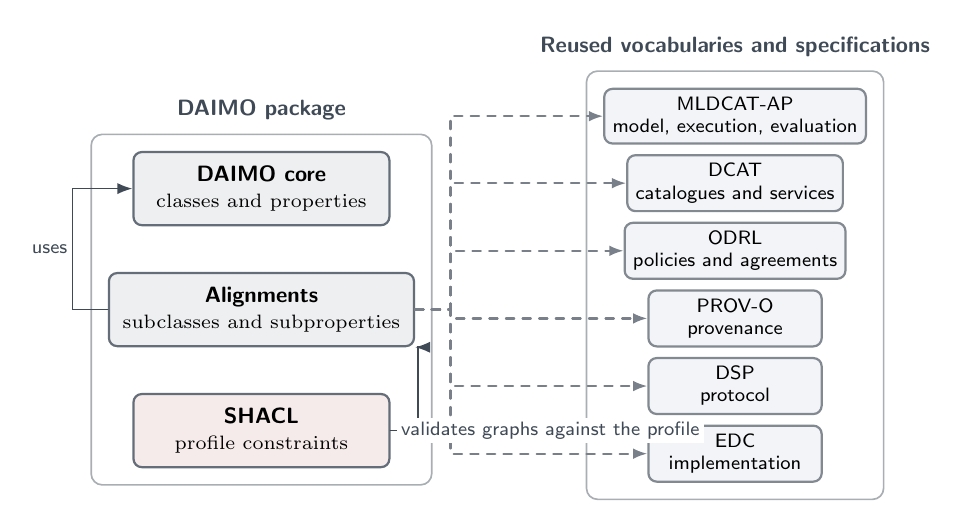
\begin{tikzpicture}[node distance=0.58cm and 1.0cm]
  \node[modulebox, minimum width=3.25cm] (core) {DAIMO core\\\scriptsize\normalfont classes and properties};
  \node[modulebox, minimum width=3.25cm, below=of core] (align) {Alignments\\\scriptsize\normalfont subclasses and subproperties};
  \node[modulebox, fill=daimoShapeFill, minimum width=3.25cm, below=of align] (shapes) {SHACL\\\scriptsize\normalfont profile constraints};

  \node[vocabbox, right=2.7cm of core, yshift=0.92cm] (mldcat) {MLDCAT-AP\\\scriptsize model, execution, evaluation};
  \node[vocabbox, below=0.12cm of mldcat] (dcat) {DCAT\\\scriptsize catalogues and services};
  \node[vocabbox, below=0.12cm of dcat] (odrl) {ODRL\\\scriptsize policies and agreements};
  \node[vocabbox, below=0.12cm of odrl] (prov) {PROV-O\\\scriptsize provenance};
  \node[vocabbox, below=0.12cm of prov] (dsp) {DSP\\\scriptsize protocol};
  \node[vocabbox, below=0.12cm of dsp] (edc) {EDC\\\scriptsize implementation};

  \draw[objpropertyarrow] (align.west) -- ++(-0.45,0) |- node[edgelabel, pos=0.25, left] {uses} (core.west);
  \draw[modulearrow] (align.east) -- ++(0.45,0) |- (mldcat.west);
  \draw[modulearrow] (align.east) -- ++(0.45,0) |- (dcat.west);
  \draw[modulearrow] (align.east) -- ++(0.45,0) |- (odrl.west);
  \draw[modulearrow] (align.east) -- ++(0.45,0) |- (prov.west);
  \draw[modulearrow] (align.east) -- ++(0.45,0) |- (dsp.west);
  \draw[modulearrow] (align.east) -- ++(0.45,0) |- (edc.west);
  \draw[objpropertyarrow] (shapes.east) -- ++(0.35,0)
    node[edgelabel, right, pos=0.2] {validates graphs against the profile}
    |- (align.south east);

  \begin{scope}[on background layer]
    \node[fit=(core)(align)(shapes), groupbox, fill=white] (daimobox) {};
    \node[above=0.05cm of daimobox, figlabel] {DAIMO package};
    \node[fit=(mldcat)(edc), groupbox, fill=white] (vocbox) {};
    \node[above=0.05cm of vocbox, figlabel] {Reused vocabularies and specifications};
  \end{scope}
\end{tikzpicture}
}
\caption{Modular organisation of the DAIMO package and reused resources.}
\label{fig:architecture}
\end{figure}

\paragraph{Artefact metrics.}\label{sec:metrics}

Before reviewing the individual classes that populate the three modules of §\ref{sec:scope}, we report the size and expressivity of the artefact globally. Table~\ref{tab:metrics} extracts the metrics directly from the Turtle files and from the reports produced by the validation suite (§\ref{sec:eval}). The numbers let an interested reader estimate the weight of the artefact before consuming it and compare it with ontologies previously published in the same family.

\begin{table}[t]
\small\sf\centering
\caption{Main DAIMO artefact metrics.\label{tab:metrics}}
\begin{tabular}{@{}p{4.6cm}r@{}}
\toprule
\textbf{Dimension} & \textbf{Value} \\
\midrule
Declared logical profile & OWL 2 DL \\
DAIMO top-level classes & 9 \\
DAIMO subclasses (\code{ParticipantRole}) & 5 \\
Total DAIMO-specific classes & 14 \\
Object properties (\code{owl:ObjectProperty}) & 29 \\
Datatype properties (\code{owl:DatatypeProperty}) & 8 \\
Functional properties (\code{owl:FunctionalProperty}) & 27 \\
Asymmetric properties (\code{owl:AsymmetricProperty}) & 5 \\
Explicit inverse pairs (\code{owl:inverseOf}) & 5 \\
\code{rdfs:subClassOf} to externals & 8 \\
\code{rdfs:subPropertyOf} to externals & 6 \\
Named disjointness axiom & 1 \\
Total \code{sh:NodeShape}s & 18 \\
\quad completeness (one per DAIMO class) & 9 \\
\quad conformance over reused classes & 3 \\
\quad cross-class SPARQL invariants & 6 \\
Competency questions & 23 \\
OOPS! pitfalls (Critical/Important/Minor) & 0 / 0 / 2 \\
\bottomrule
\end{tabular}
\end{table}

To make those counts auditable, an OntoMetrics-style breakdown is kept separate from the summary above. The distinction is useful because it avoids inflating the figures with external declarations loaded only for alignment and makes clear what is counted as a DAIMO-native term.

\begin{table}[t]
\small\sf\centering
\caption{OntoMetrics breakdown restricted to the DAIMO namespace.\label{tab:ontometrics}}
\begin{tabular}{@{}p{5.0cm}r@{}}
\toprule
\textbf{Axiom / declaration type} & \textbf{Count} \\
\midrule
\code{owl:Class} declarations, DAIMO-native & 14 \\
\code{owl:ObjectProperty} declarations, DAIMO-native & 29 \\
\code{owl:DatatypeProperty} declarations, DAIMO-native & 8 \\
\code{rdfs:subClassOf}, DAIMO-native subjects & 13 \\
\code{rdfs:subPropertyOf}, DAIMO-native subjects & 6 \\
\code{rdfs:domain}, DAIMO-native properties & 37 \\
\code{rdfs:range}, DAIMO-native properties & 37 \\
\code{owl:FunctionalProperty}, DAIMO-native properties & 27 \\
\code{owl:AsymmetricProperty} & 5 \\
\code{owl:inverseOf} pairs & 5 \\
\code{owl:AllDisjointClasses} named axioms & 1 \\
\code{owl:equivalentClass} & 0 \\
\code{owl:disjointWith} binary axioms & 0 \\
\bottomrule
\end{tabular}
\end{table}

The breakdown in Table~\ref{tab:ontometrics} shows that the reported figures count only DAIMO-native subjects, so the alignment declarations that link the profile to external vocabularies are not inflating the totals. The high proportion of functional properties, domains, and ranges reflects a deliberately constrained design in which most relations are typed and single-valued. The two zeros for \code{owl:equivalentClass} and binary \code{owl:disjointWith} are expected, because disjointness is expressed through a single named \code{owl:AllDisjointClasses} axiom.

\subsection{Classes and alignments}\label{sec:classes}

The nine top-level native classes, plus the five \code{ParticipantRole} subclasses, constitute the minimal set produced by the three core design decisions. Table~\ref{tab:classes} acts as an exhaustive inventory: class, alignment, role, and associated competency questions. The following figures do not duplicate that inventory; they provide a conceptual reading of the set and an axiomatic reading of the main alignments.

\begin{table*}[t]
\scriptsize\sf\centering
\caption{Native classes, axiomatic alignments, and competency questions.\label{tab:classes}}
\begin{tabular}{@{}p{4cm}p{3cm}p{6cm}p{2.2cm}@{}}
\toprule
\textbf{Class} & \textbf{Alignment} & \textbf{Role} & \textbf{CQs} \\
\midrule
\code{daimo:AIAsset}\newline\code{Offering} & \code{dcat:CatalogRecord} & Catalogue record that publishes a model as a governed offer in a dataspace; carries an ODRL policy through \code{daimo:hasOfferPolicy}. & R1, R2, R5, G1 \\
\code{daimo:ParticipantRole} \newline (+5 non-disjoint subclasses) & \code{prov:Role} & Role a participant plays with respect to an AI asset within a dataspace context. & R5 \\
\code{daimo:Model}\newline\code{Deployment} & \code{prov:Entity} & Running or hosted instance of a model, exposed as a \code{dcat:DataService} over an \code{it6:ComputerInfrastructure}. & E1, E3, G2 \\
\code{daimo:IOContract} & (no alignment) & Minimal actionable contract: I/O formats, authentication method, optional schemas. & R4, E1, G2 \\
\code{daimo:Execution}\newline\code{Authorization} & \code{odrl:Agreement} & ODRL agreement derived from a DSP negotiation that authorises concrete executions through \code{daimo:authorizesRun}. & E2, E5, G3 \\
\code{daimo:DerivedArtifact} & \code{prov:Entity}, \code{dcat:Resource} & Governed, catalogueable output produced by an execution under authorisation. & E5, G4 \\
\code{daimo:CrossParticipant}\newline\code{ProvenanceRecord} & \code{prov:Bundle} & Aggregation of activities and entities across participant contexts forming an audit narrative. & G4 \\
\code{daimo:AuditEvidence} & \code{prov:Entity} & Compliance-oriented evidence record with structured \code{spdx:Checksum}, signer, and timestamp. & E4 \\
\code{daimo:SharedEvaluation}\newline\code{Context} & (no alignment) & Reified comparability conditions: task, dataset, version, protocol, and random seed. & V1, V2, V3 \\
\bottomrule
\end{tabular}
\end{table*}

Figure~\ref{fig:ontology-global} provides a class-level reading of the profile as an ontological diagram: each box shows a class name and, where relevant, its main attributes, and the labelled arrows are the object properties that connect them. Bridge classes appear in blue, reused external classes in grey, evidence classes in amber, and the evaluation context in green, so a reader can see at a glance which concepts DAIMO introduces and which it takes from established vocabularies. The diagram is deliberately restricted to the most important classes and relations of the governed chain---publication, deployment, invocation, authorisation, execution, evidence, and evaluation---rather than reproducing every term. It should be read as the conceptual map that the rest of the section develops group by group.

\begin{figure*}[t]
\centering
\resizebox{\textwidth}{!}{%
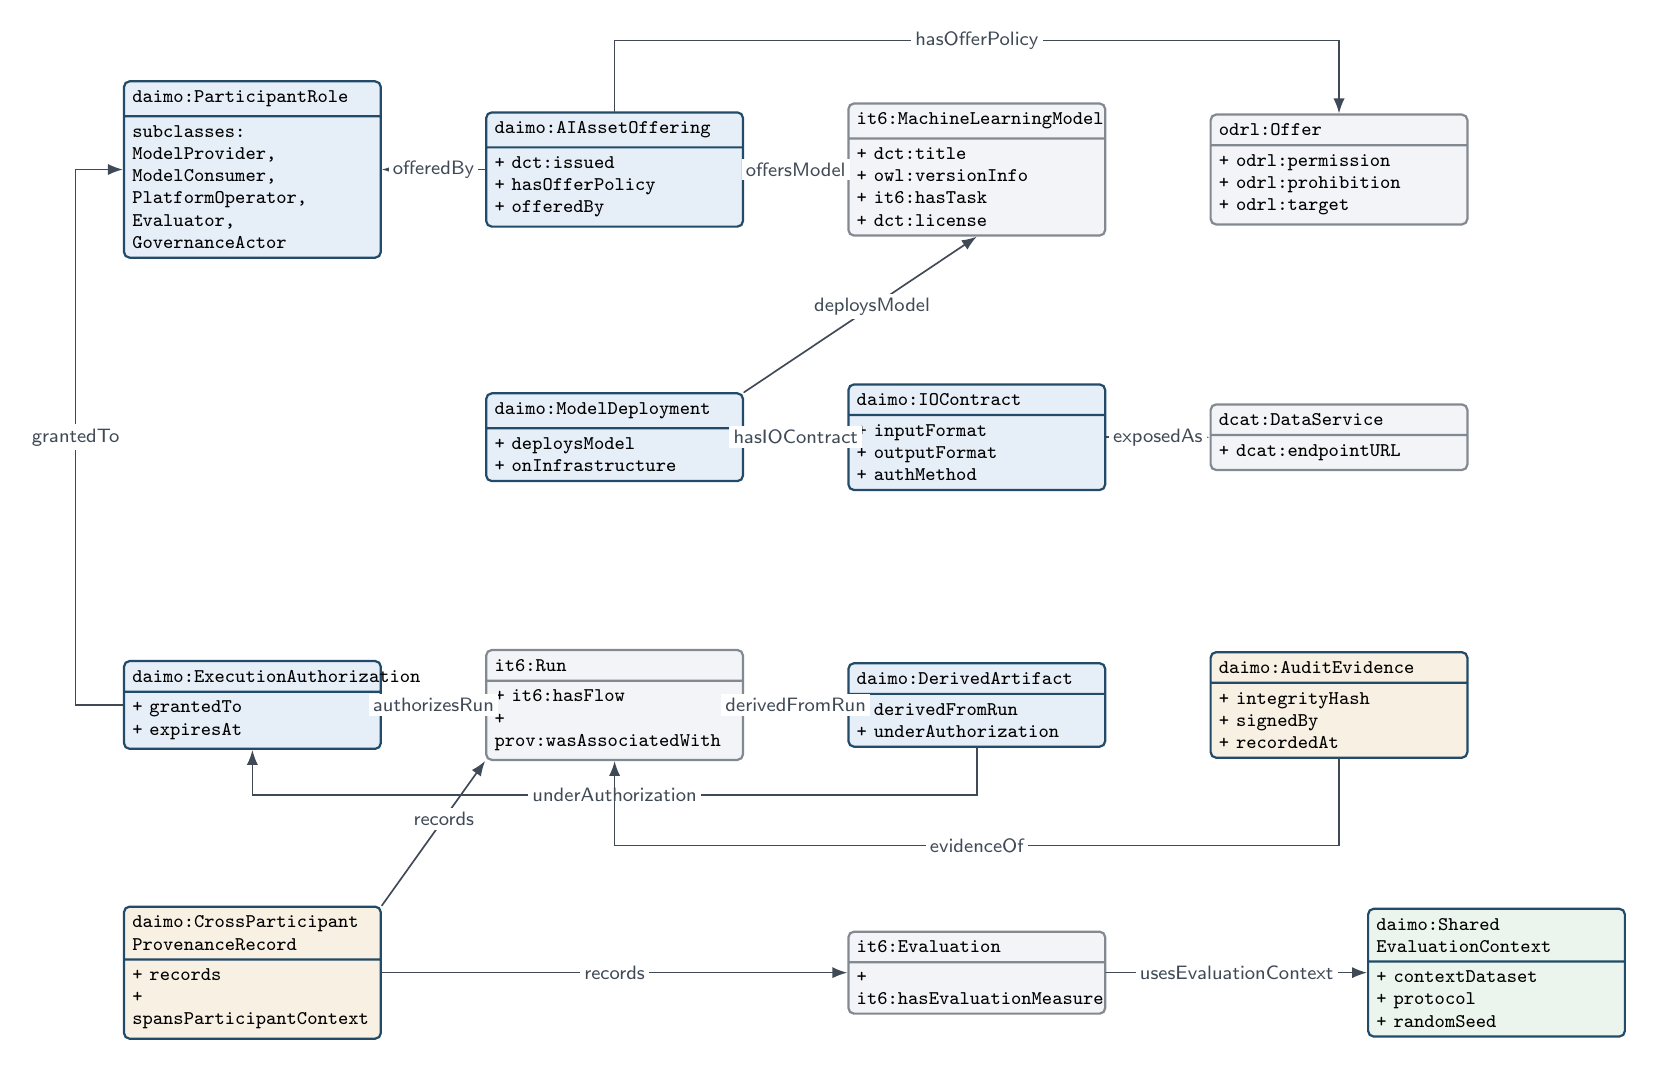
\begin{tikzpicture}[x=1cm,y=1cm]
  % --- Publication and governance row ---
  \node[umlclass] (role) at (0,0)
    {\textbf{daimo:ParticipantRole}\nodepart{two}subclasses:\\ModelProvider,\\ModelConsumer,\\PlatformOperator,\\Evaluator,\\GovernanceActor};
  \node[umlclass] (offer) at (4.6,0)
    {\textbf{daimo:AIAssetOffering}\nodepart{two}+ dct:issued\\+ hasOfferPolicy\\+ offeredBy};
  \node[umlreuse] (mlm) at (9.2,0)
    {\textbf{it6:MachineLearningModel}\nodepart{two}+ dct:title\\+ owl:versionInfo\\+ it6:hasTask\\+ dct:license};
  \node[umlreuse] (policy) at (13.8,0)
    {\textbf{odrl:Offer}\nodepart{two}+ odrl:permission\\+ odrl:prohibition\\+ odrl:target};

  % --- Deployment and invocation row ---
  \node[umlclass] (deploy) at (4.6,-3.4)
    {\textbf{daimo:ModelDeployment}\nodepart{two}+ deploysModel\\+ onInfrastructure};
  \node[umlclass] (io) at (9.2,-3.4)
    {\textbf{daimo:IOContract}\nodepart{two}+ inputFormat\\+ outputFormat\\+ authMethod};
  \node[umlreuse] (svc) at (13.8,-3.4)
    {\textbf{dcat:DataService}\nodepart{two}+ dcat:endpointURL};

  % --- Authorised execution row ---
  \node[umlclass] (auth) at (0,-6.8)
    {\textbf{daimo:ExecutionAuthorization}\nodepart{two}+ grantedTo\\+ expiresAt};
  \node[umlreuse] (run) at (4.6,-6.8)
    {\textbf{it6:Run}\nodepart{two}+ it6:hasFlow\\+ prov:wasAssociatedWith};
  \node[umlclass] (deriv) at (9.2,-6.8)
    {\textbf{daimo:DerivedArtifact}\nodepart{two}+ derivedFromRun\\+ underAuthorization};
  \node[umlevidence] (evid) at (13.8,-6.8)
    {\textbf{daimo:AuditEvidence}\nodepart{two}+ integrityHash\\+ signedBy\\+ recordedAt};

  % --- Provenance and evaluation row ---
  \node[umlevidence] (cppr) at (0,-10.2)
    {\textbf{daimo:CrossParticipant}\\\textbf{ProvenanceRecord}\nodepart{two}+ records\\+ spansParticipantContext};
  \node[umlreuse] (eval) at (9.2,-10.2)
    {\textbf{it6:Evaluation}\nodepart{two}+ it6:hasEvaluationMeasure};
  \node[umleval] (sec) at (15.8,-10.2)
    {\textbf{daimo:Shared}\\\textbf{EvaluationContext}\nodepart{two}+ contextDataset\\+ protocol\\+ randomSeed};

  % --- Object properties (associations) ---
  \draw[umlrel] (offer) -- node[edgelabel,pos=0.5]{offersModel} (mlm);
  \draw[umlrel] (offer) -- node[edgelabel,pos=0.5]{offeredBy} (role);
  \draw[umlrel] (offer.north) -- ++(0,0.9) -| node[edgelabel,pos=0.25]{hasOfferPolicy} (policy.north);
  \draw[umlrel] (deploy.north east) -- node[edgelabel,pos=0.55]{deploysModel} (mlm.south);
  \draw[umlrel] (deploy) -- node[edgelabel,pos=0.5]{hasIOContract} (io);
  \draw[umlrel] (io) -- node[edgelabel,pos=0.5]{exposedAs} (svc);
  \draw[umlrel] (auth) -- node[edgelabel,pos=0.5]{authorizesRun} (run);
  \draw[umlrel] (auth.west) -- ++(-0.6,0) |- node[edgelabel,pos=0.25]{grantedTo} (role.west);
  \draw[umlrel] (deriv) -- node[edgelabel,pos=0.5]{derivedFromRun} (run);
  \draw[umlrel] (deriv.south) -- ++(0,-0.6) -| node[edgelabel,pos=0.25]{underAuthorization} (auth.south);
  \draw[umlrel] (evid.south) -- ++(0,-1.1) -| node[edgelabel,pos=0.25]{evidenceOf} (run.south);
  \draw[umlrel] (cppr.north east) -- node[edgelabel,pos=0.6]{records} (run.south west);
  \draw[umlrel] (cppr) -- node[edgelabel,pos=0.5]{records} (eval);
  \draw[umlrel] (eval) -- node[edgelabel,pos=0.5]{usesEvaluationContext} (sec);
\end{tikzpicture}
}
\caption{Global ontological view of DAIMO: core bridge classes (blue), reused external classes (grey), evidence classes (amber), and the shared evaluation context (green), with their main attributes and object properties.}
\label{fig:ontology-global}
\end{figure*}

Figure~\ref{fig:classes} complements the global view at the axiomatic level, so that the two figures can be read together: the previous one shows what DAIMO connects, and this one shows how the connection is declared in OWL. The upper panel separates DAIMO bridge classes from the reused classes to which they attach through \code{rdfs:subClassOf}, making the alignment surface explicit. The lower panel retains only the main operational relations that articulate the profile, leaving the exhaustive term list to Table~\ref{tab:classes}. Splitting alignments and relations into two panels keeps each reading uncluttered.

\begin{figure}[tp]
\centering
\resizebox{\columnwidth}{!}{%
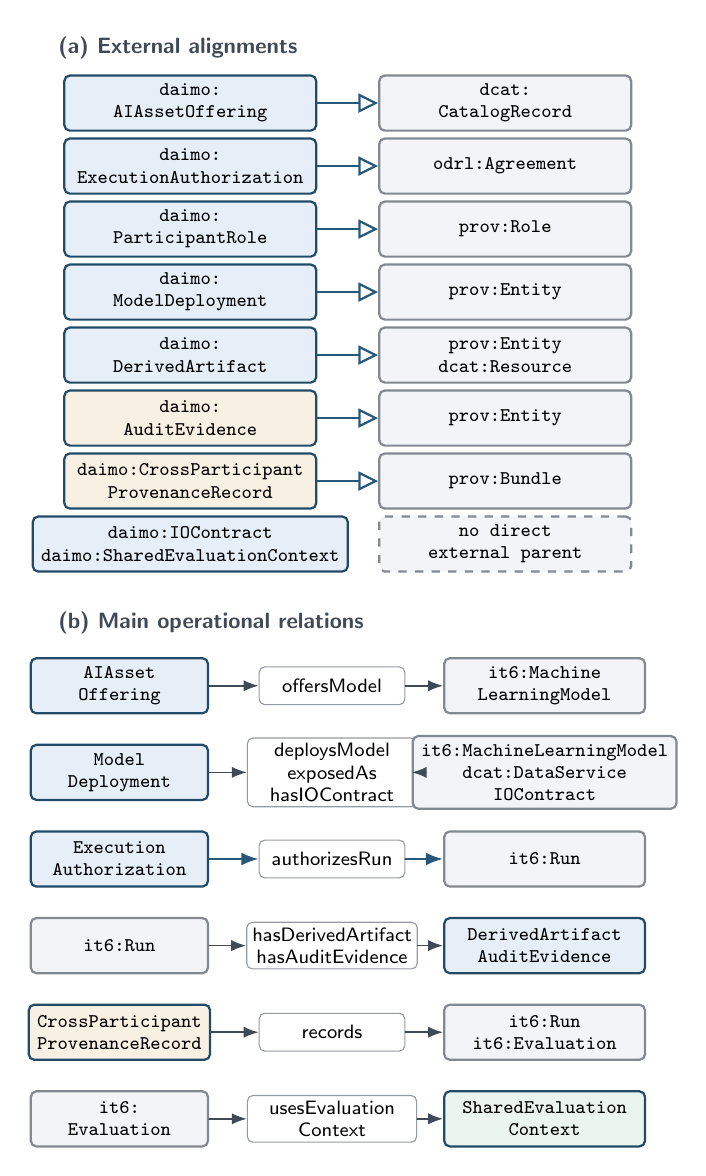
\begin{tikzpicture}[x=1cm,y=1cm,
  propbox/.style={rectangle, draw=daimoLine!55, fill=white, rounded corners=2pt,
    minimum width=1.85cm, minimum height=0.48cm, align=center,
    font=\sffamily\scriptsize, inner sep=2pt}]
  \node[figlabel, anchor=west] at (-3.6,0.25) {(a) External alignments};

  \node[daimoclass, minimum width=3.2cm] (a1) at (-1.8,-0.45) {daimo:\\AIAssetOffering};
  \node[externclass, minimum width=3.2cm] (a1t) at (2.2,-0.45) {dcat:\\CatalogRecord};
  \draw[subclassarrow] (a1) -- (a1t);

  \node[daimoclass, minimum width=3.2cm] (a2) at (-1.8,-1.25) {daimo:\\ExecutionAuthorization};
  \node[externclass, minimum width=3.2cm] (a2t) at (2.2,-1.25) {odrl:Agreement};
  \draw[subclassarrow] (a2) -- (a2t);

  \node[daimoclass, minimum width=3.2cm] (a3) at (-1.8,-2.05) {daimo:\\ParticipantRole};
  \node[externclass, minimum width=3.2cm] (a3t) at (2.2,-2.05) {prov:Role};
  \draw[subclassarrow] (a3) -- (a3t);

  \node[daimoclass, minimum width=3.2cm] (a4) at (-1.8,-2.85) {daimo:\\ModelDeployment};
  \node[externclass, minimum width=3.2cm] (a4t) at (2.2,-2.85) {prov:Entity};
  \draw[subclassarrow] (a4) -- (a4t);

  \node[daimoclass, minimum width=3.2cm] (a5) at (-1.8,-3.65) {daimo:\\DerivedArtifact};
  \node[externclass, minimum width=3.2cm] (a5t) at (2.2,-3.65) {prov:Entity\\dcat:Resource};
  \draw[subclassarrow] (a5) -- (a5t);

  \node[evidencebox, minimum width=3.2cm] (a6) at (-1.8,-4.45) {daimo:\\AuditEvidence};
  \node[externclass, minimum width=3.2cm] (a6t) at (2.2,-4.45) {prov:Entity};
  \draw[subclassarrow] (a6) -- (a6t);

  \node[evidencebox, minimum width=3.2cm] (a7) at (-1.8,-5.25) {daimo:CrossParticipant\\ProvenanceRecord};
  \node[externclass, minimum width=3.2cm] (a7t) at (2.2,-5.25) {prov:Bundle};
  \draw[subclassarrow] (a7) -- (a7t);

  \node[daimoclass, minimum width=3.2cm] (a8) at (-1.8,-6.05) {daimo:IOContract\\daimo:SharedEvaluationContext};
  \node[externclass, minimum width=3.2cm, dashed] (a8t) at (2.2,-6.05) {no direct\\external parent};

  \node[figlabel, anchor=west] at (-3.6,-7.05) {(b) Main operational relations};

  \node[daimoclass, minimum width=2.25cm] (b1) at (-2.7,-7.85) {AIAsset\\Offering};
  \node[propbox] (b1p) at (0,-7.85) {offersModel};
  \node[externclass, minimum width=2.55cm] (b1t) at (2.7,-7.85) {it6:Machine\\LearningModel};
  \draw[objpropertyarrow] (b1) -- (b1p);
  \draw[objpropertyarrow] (b1p) -- (b1t);

  \node[daimoclass, minimum width=2.25cm] (b2) at (-2.7,-8.95) {Model\\Deployment};
  \node[propbox, minimum width=2.15cm] (b2p) at (0,-8.95) {deploysModel\\exposedAs\\hasIOContract};
  \node[externclass, minimum width=2.55cm] (b2t) at (2.7,-8.95) {it6:MachineLearningModel\\dcat:DataService\\IOContract};
  \draw[objpropertyarrow] (b2) -- (b2p);
  \draw[objpropertyarrow] (b2p) -- (b2t);

  \node[daimoclass, minimum width=2.25cm] (b3) at (-2.7,-10.05) {Execution\\Authorization};
  \node[propbox] (b3p) at (0,-10.05) {authorizesRun};
  \node[externclass, minimum width=2.55cm] (b3t) at (2.7,-10.05) {it6:Run};
  \draw[flowarrow] (b3) -- (b3p);
  \draw[flowarrow] (b3p) -- (b3t);

  \node[externclass, minimum width=2.25cm] (b4) at (-2.7,-11.15) {it6:Run};
  \node[propbox, minimum width=2.15cm] (b4p) at (0,-11.15) {hasDerivedArtifact\\hasAuditEvidence};
  \node[daimoclass, minimum width=2.55cm] (b4t) at (2.7,-11.15) {DerivedArtifact\\AuditEvidence};
  \draw[objpropertyarrow] (b4) -- (b4p);
  \draw[objpropertyarrow] (b4p) -- (b4t);

  \node[evidencebox, minimum width=2.25cm] (b5) at (-2.7,-12.25) {CrossParticipant\\ProvenanceRecord};
  \node[propbox] (b5p) at (0,-12.25) {records};
  \node[externclass, minimum width=2.55cm] (b5t) at (2.7,-12.25) {it6:Run\\it6:Evaluation};
  \draw[objpropertyarrow] (b5) -- (b5p);
  \draw[objpropertyarrow] (b5p) -- (b5t);

  \node[externclass, minimum width=2.25cm] (b6) at (-2.7,-13.35) {it6:\\Evaluation};
  \node[propbox, minimum width=2.15cm] (b6p) at (0,-13.35) {usesEvaluation\\Context};
  \node[evalbox, minimum width=2.55cm] (b6t) at (2.7,-13.35) {SharedEvaluation\\Context};
  \draw[objpropertyarrow] (b6) -- (b6p);
  \draw[objpropertyarrow] (b6p) -- (b6t);
\end{tikzpicture}
}
\caption{External alignments and main DAIMO relations.}
\label{fig:classes}
\end{figure}

The following paragraphs explain the modelling decisions by function. They do not repeat the full traceability of Table~\ref{tab:classes}; they concentrate on why each grouping exists and which semantic boundary it preserves.

\medskip\noindent\emph{Publication and governance.}\par\nobreak\noindent
\code{AIAssetOffering} represents the act of registering a model as a governed offer in a dataspace catalogue. The class does not replace the model: the model remains \code{it6:MachineLearningModel}, reused from MLDCAT-AP, and the offering only contextualises its publication with provider, ODRL policy, and catalogue metadata. \code{ParticipantRole} captures the contextual role an agent plays with respect to the asset; its five subclasses (\code{ModelProvider}, \code{ModelConsumer}, \code{PlatformOperator}, \code{Evaluator}, and \code{GovernanceActor}) are not disjoint, because one agent may play several roles in different contexts. The profile is not a catalogue of catalogues: it models only the governed offering of AI models within the exchange described.

\medskip\noindent\emph{Deployment and invocation.}\par\nobreak\noindent
\code{ModelDeployment} and \code{IOContract} connect the reused model to the invocation point. The deployment identifies the hosted or running instance of the model and may be exposed through one or several \code{dcat:DataService}s; the I/O contract describes formats, authentication, and optional schema references. DAIMO records where and under which syntactic conditions a model can be invoked, but it does not implement the runtime, enforcement engine, container orchestration, or TEE mechanisms. It also does not by itself resolve fine-grained semantic compatibility between input and output schemas; that verification belongs to dataspace-specific profiles or shapes.

\medskip\noindent\emph{Authorisation and derived artefacts.}\par\nobreak\noindent
\code{ExecutionAuthorization} reifies the agreement that authorises concrete executions, relying on ODRL for permissions and restrictions, and \code{DerivedArtifact} represents the governable output produced by an \code{it6:Run}. This separation avoids conflating three planes: negotiated policy, execution activity, and produced result. DAIMO describes the semantic chain that lets one ask under which authorisation an artefact was produced; it does not model the operational mechanism that decides or executes access.

\medskip\noindent\emph{Evidence and provenance.}\par\nobreak\noindent
\code{AuditEvidence} records verifiable evidence about an activity through integrity, signer, and timestamp; \code{CrossParticipantProvenanceRecord} aggregates activities and entities across participant contexts to form an audit narrative. PROV-O supplies the entity--activity--bundle pattern; SPDX supplies the structured checksum. DAIMO does not claim automatic compliance or external validation of that evidence: it provides the relations needed for evidence to be represented and queried.

\medskip\noindent\emph{Shared evaluation.}\par\nobreak\noindent
\code{SharedEvaluationContext} reifies the conditions that make two evaluations comparable: task, dataset, version, protocol, and seed. Measurements remain \code{it6:Evaluation} and \code{it6:EvaluationMeasure}; DAIMO adds only the context that prevents interpreting a metric as an absolute property of the model. This decision keeps a universal theory of bias, fairness, explainability, or security outside the core: those dimensions can be expressed as contextualised measures or specialised profiles when a use case requires them.

\medskip\noindent\emph{Compact alignment defence.}\label{sec:alignment-defense}\par\nobreak\noindent
External alignments follow the same minimal-duplication criterion. \code{AIAssetOffering} aligns with \code{dcat:CatalogRecord}, not \code{dcat:Dataset}, because the offering is the contextual record that describes a model in a catalogue, not the model or a dataset; \code{offersModel} maintains the link to \code{it6:MachineLearningModel}. \code{ExecutionAuthorization} aligns with \code{odrl:Agreement} because the authorisation is the effective agreement that covers executions, not a derived artefact of another agreement. \code{ParticipantRole} aligns with \code{prov:Role} with caution: DAIMO adds administrative scope through participant context, but preserves the reading of role as a contextual qualification of participation.

The remaining alignments preserve the PROV-O entity--activity distinction. \code{ModelDeployment} is a \code{prov:Entity}, not an activity; \code{DerivedArtifact} is both \code{prov:Entity} and \code{dcat:Resource}, because it is produced by a run and can be catalogued; \code{CrossParticipantProvenanceRecord} is a \code{prov:Bundle}, not a generic collection; and \code{AuditEvidence} is a \code{prov:Entity}, not the act of auditing. \code{IOContract} and \code{SharedEvaluationContext} have no direct external parent by design: the former is neither a service nor a standard, and the latter is not a task or an evaluation, but the reification of comparability conditions.


\subsection{Axiomatic foundations}\label{sec:axiomatic}

A taxonomy alone does not fix meaning; it only names the types. DAIMO therefore combines the class hierarchy with an axiomatic infrastructure that fixes what each class is, what it is not, and how conforming instances must behave. Three complementary strata make up this infrastructure: OWL axioms over classes and properties, SHACL nodal constraints over instances, and SHACL-SPARQL cross-class invariants. The OWL stratum is described here; the SHACL strata are reported in Section~\ref{sec:eval} as part of validation.

On the OWL stratum, disjointness between the nine DAIMO top-level kinds is declared through the named axiom \code{daimo:TopLevelKindsDisjointness}, an instance of \code{owl:AllDisjointClasses}. The five \code{ParticipantRole} subclasses are deliberately excluded: one legal agent may hold several roles at once (provider and operator, for instance), which reflects that roles are context-dependent rather than mutually exclusive.

The disjointness core is complemented by property characterisations. Twenty-seven properties are declared functional where the corresponding structural shape also imposes maximum cardinality, so cardinality is represented in both the logical and validation layers. Five lifecycle relations are asymmetric, which formally captures that a deployment is not the model it deploys, an authorisation does not coincide with the execution it authorises, and so on. Five inverse pairs support bidirectional traversal without forcing the publisher of the graph to materialise both directions.

The SHACL stratum splits into two families. Each DAIMO governance class carries a structural nodal shape that prescribes which properties are mandatory in a well-formed instance; these nine shapes are the syntactic guarantee that a publisher has supplied everything the semantic invariants need. Three conformance shapes (\code{OfferInDAIMOShape}, \code{MachineLearningModelInDAIMOShape}, and \code{RunInDAIMOShape}) establish which properties of reused classes are mandatory when a graph declares adherence to the DAIMO profile. The distinction between the two families is intentional: DAIMO does not override the underlying ontology, because that would fracture the ecosystem. Instead, it declares a commitment to a concrete subset of properties on the external classes, making the adherence criterion explicit without modifying the original definitions.

Above the shapes sit the six SHACL-SPARQL cross-class invariants (INV-1 through INV-6), examined in detail during validation. They encode rules whose meaning cannot be expressed as a local constraint on a single shape because the rules span several classes simultaneously. Listing~\ref{lst:axioms} shows how the OWL axioms are encoded for the concrete case of \code{ExecutionAuthorization}: the subclass of \code{odrl:Agreement}, the asymmetry of \code{authorizesRun}, the functionality of its inverse, and membership in the named disjointness axiom.

\begin{lstlisting}[label=lst:axioms,caption={Core axioms around \code{ExecutionAuthorization}.}]
daimo:ExecutionAuthorization a owl:Class ;
    rdfs:subClassOf odrl:Agreement ;
    skos:definition "An ODRL agreement produced by a DSP contract
        negotiation that binds specific permissions to run invocations..."@en .

daimo:authorizesRun a owl:ObjectProperty , owl:AsymmetricProperty ;
    rdfs:domain daimo:ExecutionAuthorization ;
    rdfs:range  it6:Run .

daimo:authorizedBy a owl:ObjectProperty , owl:FunctionalProperty ;
    owl:inverseOf daimo:authorizesRun ;
    rdfs:domain it6:Run ;
    rdfs:range  daimo:ExecutionAuthorization .

daimo:TopLevelKindsDisjointness a owl:AllDisjointClasses ;
    owl:members ( daimo:AIAssetOffering
                  daimo:ExecutionAuthorization
                  daimo:ModelDeployment
                  daimo:DerivedArtifact
                  daimo:IOContract
                  daimo:AuditEvidence
                  daimo:CrossParticipantProvenanceRecord
                  daimo:SharedEvaluationContext
                  daimo:ParticipantRole ) .
\end{lstlisting}

\medskip\noindent\emph{Reuse surface.}\label{sec:reuse}
Table~\ref{tab:reuse} summarises the reused vocabularies and their concrete use. Three observations matter. First, the alignments to DCAT and ODRL target standard vocabularies rather than implementation-internal entities. Second, DAIMO maintains informative mappings to DSP through \code{skos:closeMatch} and \code{skos:related}, not subsumption: DSP is a messaging protocol rather than an asset ontology, and subsuming DAIMO classes under DSP constructs would introduce spurious typings. Third, of the EDC extension only \code{edc:ParticipantContext} appears explicitly, where it anchors aggregated provenance to an administrative context.

\begin{table*}[t]
\small\sf\centering
\caption{Vocabularies reused by DAIMO and the concrete use of each.\label{tab:reuse}}
\begin{tabular}{@{}p{2.6cm}p{5cm}p{7cm}@{}}
\toprule
\textbf{Vocabulary} & \textbf{Reused terms} & \textbf{Use in DAIMO} \\
\midrule
MLDCAT-AP 3.0.0 (\code{it6:}) & \code{MachineLearningModel}, \code{Task}, \code{Run}, \code{Flow}, \code{Evaluation}, \code{EvaluationMeasure}, \code{Benchmark}, \code{ComputerInfrastructure}, \code{Hardware}, \code{Library}, \code{HarmRisk}, \code{Modality}, \code{trainedOn}, \code{testedOn} & AI-asset plane; DAIMO does not redefine the model. \\
DCAT 2 (\code{dcat:}) & \code{Catalog}, \code{Dataset}, \code{Distribution}, \code{DataService}, \code{CatalogRecord}, \code{endpointURL} & Publication and discovery. \\
ODRL 2.2 (\code{odrl:}) & \code{Offer}, \code{Agreement}, \code{Permission}, \code{Prohibition}, \code{hasPolicy}, \code{target}, \code{assigner}, \code{assignee} & Policy, offer, and agreement. \\
PROV-O (\code{prov:}) & \code{Activity}, \code{Entity}, \code{Agent}, \code{Bundle}, \code{Role}, \code{wasGeneratedBy}, \code{wasAssociatedWith} & Provenance and roles. \\
FOAF (\code{foaf:})~\cite{foaf} & \code{primaryTopic} & Subproperty target for linking an offering record to the model it is about. \\
SPDX (\code{spdx:})~\cite{spdx} & \code{Checksum}, \code{algorithm}, \code{checksumValue} & Audit-evidence integrity. \\
SKOS (\code{skos:})~\cite{skos} & \code{definition}, \code{example}, \code{closeMatch}, \code{related} & Term documentation and non-subsumptive mappings. \\
DSP (\code{dspace:}) & \code{ContractOffer}, \code{ContractNegotiation}, \code{TransferProcess} & Informative \code{skos:closeMatch}/\code{skos:related} mappings; not subsumption. \\
EDC (\code{edc:}) & \code{ParticipantContext} & Only EDC-specific extension referenced. \\
\bottomrule
\end{tabular}
\end{table*}

Three subproperties that might seem natural (\code{authorizesRun} $\sqsubseteq$ \code{prov:used}; \code{grantedTo} $\sqsubseteq$ \code{prov:qualifiedAssociation}; \code{evidenceOf} $\sqsubseteq$ \code{prov:hadActivity}) are deliberately not declared, because each would produce unintended typings on authorisations, agents, or evidence under RDFS closure. The entailment-verification check reported below catches errors of this kind.

% =====================================================================
\section{Evaluation}\label{sec:eval}

Evaluation distinguishes two objects: DAIMO as an ontology artefact and the comparative evaluation of models that DAIMO can describe. The former is examined technically through formal consistency, OWL-RL closure, SHACL conformance, absence of critical pitfalls, alignment behaviour, and competency-question answering. The latter appears only inside the demonstrator as represented content under a shared context; it does not constitute an empirical benchmark of real models. The reported evidence is therefore executable over the artefact and over a controlled graph, not external expert validation or production deployment.

In LOT terms, fit-for-purpose adequacy is addressed in a bounded way through a realistic instance graph, executable SPARQL queries, and negative tests. Following the usual distinction between requirements coverage, formal correctness, constraint-based validation, and applied usefulness~\cite{brank05}, we ask whether the profile represents the target exchange, whether the OWL artefact is formally coherent, whether SHACL constraints discriminate valid from invalid graphs, and whether the competency questions are executable over the materialised graph. The analysis follows the five-dimension pattern of RePlanIT~\cite{kurteva}: scenario instantiation (§\ref{sec:eval-usecase}), formal verification through reasoning, entailment checking, and OOPS! scanning (§\ref{sec:eval-engineering}), SHACL instance validation (§\ref{sec:eval-invariants}), execution of the twenty-three competency questions (§\ref{sec:eval-cqs}), and verification of reuse alignments (§\ref{sec:eval-reuse}). All five dimensions are reproducible with the evaluation package that accompanies the artefact.

\subsection{Illustrative demonstrator}\label{sec:eval-usecase}

The PIONERA scenario introduced in §\ref{sec:scenario} is instantiated on DAIMO as a controlled demonstrator. The resulting graph contains 225 data triples that exercise every native class at least once and over which the twenty-three competency queries reported in §\ref{sec:eval-cqs} are executed. All organisations, model names, dataset versions, metrics, and endpoints are anonymised or synthetic, so the demonstrator instantiates the PIONERA case conceptually rather than mirroring any deployed instance. The demonstrator is not a deployment study, a gold standard, or a validation against real model catalogues; its function is to examine representational adequacy and make the validation artefacts executable.

The Company connector publishes three governed model offerings in the PIONERA federated catalogue: two versions of the same Mobility delay-prediction model and one read-only variant with a stricter policy. The offerings share task and domain descriptions but differ in the permissions attached to them. This part of the scenario exercises the distinction between a model as an AI asset and an offering as a contextual catalogue record with its own usage conditions.

The selected Mobility model is deployed on a described compute environment and exposed through two service interfaces: a REST endpoint with JSON input and bearer-token authentication, and a gRPC endpoint with protobuf and mutual TLS. The multi-endpoint usage exercises the modelling decision that a single deployment may expose several services and contracts, rather than forcing one endpoint per deployment.

The City Council connector obtains an execution authorisation with explicit validity dates, invokes the model, and receives a derived prediction artefact. The execution is linked to audit evidence containing an integrity record, signer, and timestamp, so that a governance actor can reconstruct how the artefact was produced and under which authorisation. A cross-participant provenance record aggregates the chain across the Company, City Council, and platform contexts. A PIONERA benchmarking service publishes two synthetic evaluation results under the same benchmark, protocol, and random seed, allowing the two model versions to be compared under shared conditions.

Figure~\ref{fig:scenario} summarises the demonstrator as a phase flow. The phases are read from top to bottom, from publication to shared evaluation, and each retains only the constructs needed to explain DAIMO's representational role. Fine-grained property detail remains in the text and in the query traceability.

\begin{figure}[H]
\centering
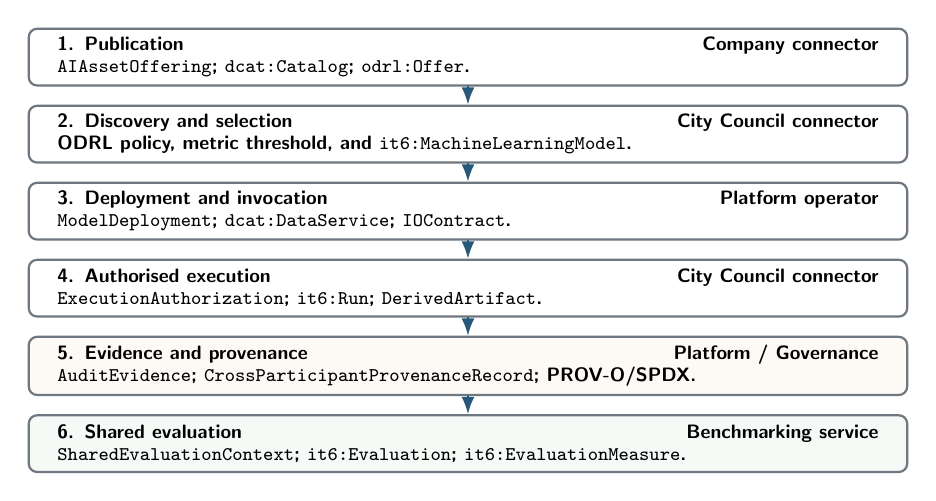
\begin{tikzpicture}[node distance=0.23cm]
  \node[phasebox, text width=0.86\columnwidth, minimum width=0.92\columnwidth,
    align=left, fill=white] (s1)
    {\textbf{1. Publication} \hfill Company connector\\
    \code{AIAssetOffering}; \code{dcat:Catalog}; \code{odrl:Offer}.};

  \node[phasebox, text width=0.86\columnwidth, minimum width=0.92\columnwidth,
    align=left, fill=white, below=of s1] (s2)
    {\textbf{2. Discovery and selection} \hfill City Council connector\\
    ODRL policy, metric threshold, and \code{it6:MachineLearningModel}.};

  \node[phasebox, text width=0.86\columnwidth, minimum width=0.92\columnwidth,
    align=left, fill=white, below=of s2] (s3)
    {\textbf{3. Deployment and invocation} \hfill Platform operator\\
    \code{ModelDeployment}; \code{dcat:DataService}; \code{IOContract}.};

  \node[phasebox, text width=0.86\columnwidth, minimum width=0.92\columnwidth,
    align=left, fill=white, below=of s3] (s4)
    {\textbf{4. Authorised execution} \hfill City Council connector\\
    \code{ExecutionAuthorization}; \code{it6:Run}; \code{DerivedArtifact}.};

  \node[phasebox, text width=0.86\columnwidth, minimum width=0.92\columnwidth,
    align=left, fill=daimoEvidenceFill!35, below=of s4] (s5)
    {\textbf{5. Evidence and provenance} \hfill Platform / Governance\\
    \code{AuditEvidence}; \code{CrossParticipantProvenanceRecord}; PROV-O/SPDX.};

  \node[phasebox, text width=0.86\columnwidth, minimum width=0.92\columnwidth,
    align=left, fill=daimoEvalFill!45, below=of s5] (s6)
    {\textbf{6. Shared evaluation} \hfill Benchmarking service\\
    \code{SharedEvaluationContext}; \code{it6:Evaluation}; \code{it6:EvaluationMeasure}.};

  \draw[flowarrow] (s1.south) -- (s2.north);
  \draw[flowarrow] (s2.south) -- (s3.north);
  \draw[flowarrow] (s3.south) -- (s4.north);
  \draw[flowarrow] (s4.south) -- (s5.north);
  \draw[flowarrow] (s5.south) -- (s6.north);
\end{tikzpicture}
\caption{Phase-based view of the bounded multi-participant demonstrator.}
\label{fig:scenario}
\end{figure}

\subsection{Formal verification}\label{sec:eval-engineering}

HermiT, invoked through \code{owlready2}, confirms that the union of the core, the alignments, and the example graph is logically consistent with no unsatisfiable classes; reasoning takes 1.25~s. OWL-RL materialisation (the \code{owlrl} library) derives 1\,170 additional triples on top of 818 initial ones (1\,988 in total) in 0.58~s, with no individuals typed as \code{owl:Nothing} and no unsatisfiable subclasses.

Logical consistency is necessary but not sufficient. An ontology may be consistent and still infer, for instance, that audit evidence is a provenance activity rather than an entity produced by an activity. We therefore added an entailment-verification check over the OWL-RL closure: for each DAIMO class, the check enumerates every inferred superclass and tests it against a list of forbidden ones. The report covers the fourteen DAIMO classes (nine top-level plus five role subclasses) and raises no warning. This check complements consistency reasoning by detecting modelling-inappropriate alignments that remain logically satisfiable.

The OOPS! scanner~\cite{oops14}, queried through its REST API on the union of the core and alignments, reports zero Critical pitfalls, zero Important ones, and two Minor ones: P13 (``inverse relationships not declared'') on 34 elements with no semantically meaningful inverse, and P04 (``isolated ontology elements'') on seven locally declared external classes. Both arise from the reuse-by-default discipline the profile applies.

Structural-quality metrics are treated as diagnostic signals, not as absolute acceptance criteria. Counts such as hierarchy depth, taxonomic breadth, connectivity, explicit equivalences, or isolated elements help identify areas that deserve inspection, but they do not by themselves prescribe a modelling change. In OWL, a \code{rdfs:subClassOf} cycle may express implicit equivalence rather than an error; an \code{owl:equivalentClass} declaration may be a legitimate alignment; and disjointness should be introduced only when the ontological commitment is true in every admissible model of the domain. DAIMO therefore uses OOPS!, HermiT, OWL-RL, SHACL, negative tests, and competency questions as complementary layers: each observes a different risk, and none replaces modelling judgement.

\subsection{SHACL validation: structural, invariants, and negative test bench}\label{sec:eval-invariants}

The SHACL layer contains three \emph{shape} families, each answering a different validation question. Structural shapes ask whether every DAIMO-specific instance carries the mandatory properties of its class. Conformance shapes ask whether reused external classes satisfy the additional obligations that the profile imposes on them. SPARQL invariants ask whether relations among offering, policy, deployment, authorisation, run, derived artefact, and evidence remain coherent. Together, the three families move validation from local completeness to graph-level consistency: from ``is this instance well-formed?'' to ``is this graph internally coherent?''. The SHACL layer therefore acts as the profile's data contract; it does not introduce a parallel ontology or require universal lineage, model-format, or metric constraints that are not justified by the competency questions.

At implementation level, constraints are encoded as \code{sh:NodeShape}s targeting DAIMO classes or reused classes under the profile, and as embedded \code{sh:PropertyShape}s that fix cardinalities, datatypes, expected classes, patterns, or closed enumerations. In an operational flow, a provider may publish RDF or JSON-LD metadata for a model, a connector or catalogue service may execute the \code{daimo-shapes.ttl} layer, and the resulting \code{sh:ValidationReport} would indicate whether the graph conforms or which specific property violates the profile. This describes the expected consumption mode of the shapes; it is not presented as an already deployed production connector or as validation of the ontology TBox itself.

The nine structural shapes impose minimum completeness per class; the positive graph of 225 triples satisfies \code{conforms=True}. The three conformance shapes add operational obligations over reused classes: \code{OfferInDAIMOShape} requires every \code{odrl:Offer} used in DAIMO to declare \code{odrl:assigner} and \code{odrl:target}; \code{MachineLearningModelInDAIMOShape} requires policy, title, and identifier on \code{it6:MachineLearningModel}; and \code{RunInDAIMOShape} requires flow, algorithm, associated agent, and timestamp on \code{it6:Run}. Additionally, \code{sh:in} restricts \code{daimo:authMethod} to a closed vocabulary of nine tokens, and \code{sh:pattern} restricts \code{daimo:protocol} to recognised evaluation-protocol names.

Above this structural stratum sit the six SHACL-SPARQL cross-class invariants. INV-1 guarantees consistency of the derivation-authorisation chain: every derived artefact must point to an authorisation that covers precisely the execution from which the artefact was derived. INV-2 requires the actor recorded in provenance for an execution to match the beneficiary in at least one covering authorisation. INV-3 checks data-plane coherence: a service exposed by a deployment must serve the same model the deployment declares, ruling out an endpoint that advertises one model and serves another. INV-4 ensures that an authorisation cannot justify an execution that started after the authorisation lapsed. INV-5 requires the policy attached to an offering to govern the model named in that offering. INV-6 closes the same triangle on the provider side by checking consistency between the catalogue-record attribution and the policy assigner. The positive graph conforms to all six invariants without warnings.

Listing~\ref{lst:inv5} shows the concrete encoding of INV-5 as \code{sh:SPARQLConstraint}, illustrating the \code{FILTER NOT EXISTS} pattern that captures the disjunction between policy-level and per-permission targets.

\begin{lstlisting}[label=lst:inv5,caption={INV-5 encoded as a \code{sh:SPARQLConstraint}.}]
daimo:OfferingPolicyTargetInvariant a sh:NodeShape ;
    sh:targetClass daimo:AIAssetOffering ;
    sh:sparql [
        a sh:SPARQLConstraint ;
        sh:message "INV-5 violation: offering's offersModel does not
                    appear as odrl:target of the attached policy."@en ;
        sh:prefixes daimo:_invariantPrefixes ;
        sh:select """
            SELECT $this ?model ?policy WHERE {
                $this daimo:offersModel ?model ;
                      daimo:hasOfferPolicy ?policy .
                FILTER NOT EXISTS { ?policy odrl:target ?model }
                FILTER NOT EXISTS { ?policy odrl:permission/odrl:target ?model }
            }
        """ ;
    ] .
\end{lstlisting}

Shapes that conform on the positive graph are necessary but not sufficient to show that constraints are semantically discriminating. For this reason DAIMO also includes a negative graph of 118 triples encoding six deliberately invalid cases---\code{bad:INV1-artifact}, \code{bad:INV2-run}, \code{bad:INV3-deployment}, \code{bad:INV4-auth}, \code{bad:INV5-offering}, and \code{bad:INV6-offering}---each focused on one invariant. The test loads the ontology, shapes, and negative graph, runs SHACL, and verifies that validation fails globally and that each expected focus node appears in the report with the specific invariant message. All six invariants fire correctly on their corresponding violation.

\subsection{Competency questions}\label{sec:eval-cqs}

The twenty-three competency questions are expressed as SPARQL queries and run over the OWL-RL materialised closure of the positive graph. The table below summarises coverage by category and preserves the observed row counts; row-level traceability appears in Table~\ref{tab:cq-trace} in Appendix~\ref{app:sparql}. All 23/23 queries return at least one row, verifying that the demonstration graph contains the information needed to answer every question with the primitives DAIMO declares; it does not evaluate the empirical quality of the models represented.

\begin{table*}[t]
\scriptsize\sf\centering
\caption{Coverage of the 23 competency questions over the positive graph closed with OWL-RL.\label{tab:cqs}}
\begin{tabular}{@{}p{3.3cm}p{2.6cm}p{0.8cm}p{6.3cm}@{}}
\toprule
\textbf{Category} & \textbf{Queries (rows)} & \textbf{N} & \textbf{Relevant semantic operation or SPARQL} \\
\midrule
Registration and publication (R) & R1(3) R2(1) R3(1) R4(2) R5(2) & 5 & \textbf{R2} (\code{subPropertyOf} chain), \textbf{R5} (\code{subClassOf} path) \\
Discovery and selection (D) & D1(3) D2(2) D3(4) D4(1) & 4 & D2 uses negation-as-failure; D4 applies a numeric filter. D1 and D3 are direct queries. \\
Execution and auditability (E) & E1(4) E2(1) E3(2) E4(1) E5(1) & 5 & \textbf{E1} (\code{offersModel}~$\sqsubseteq$~\code{foaf:primaryTopic}); E2 uses an agreement--run union. \\
Evaluation and reproducibility (V) & V1(1) V2(1) V3(2) V4(1) V5(4) & 5 & V2 uses \code{MAX} aggregation; V3 uses ordering. \\
Governance bridge (G) & G1(1) G2(2) G3(1) G4(1) & 4 & G3 exercises the DAIMO--ODRL bridge; G4 uses \code{GROUP\_CONCAT}. \\
\bottomrule
\end{tabular}
\end{table*}

Two results deserve emphasis. CQ-R2 and CQ-E1 depend on the \code{subPropertyOf} relation between \code{daimo:offersModel} and \code{foaf:primaryTopic} and return no rows on a plain SPARQL engine without reasoning; CQ-R5 explicitly traverses the role hierarchy. The dependency is documented, not a defect: aligning \code{offersModel} under \code{foaf:primaryTopic} makes offerings discoverable through the standard DCAT descriptive property, a benefit that materialises only under inference. A consumer who needs to run those queries on a plain endpoint can materialise the closure beforehand or rewrite the queries to enumerate both properties. The second result is that CQ-G2 returns two rows---one per endpoint of the multi-protocol REST and gRPC deployment---confirming that modelling several services per deployment is representable and directly queryable from SPARQL.

Two fragments illustrate the formalisation pattern. Listing~\ref{lst:cq-g3} shows CQ-G3: the query retrieves the authorisation that covers a concrete run, the authorised grantee, and the expiry time. The alignment \code{ExecutionAuthorization}~$\sqsubseteq$~\code{odrl:Agreement} makes the resource interpretable as an ODRL agreement without duplicating contract properties in the query. Listing~\ref{lst:cq-v3} shows CQ-V3: two evaluations are compared only because they share the same \code{SharedEvaluationContext}; ordering by metric value is meaningful inside that context rather than as a global ranking independent of dataset, protocol, or seed.

\begin{lstlisting}[label=lst:cq-g3,caption={CQ-G3: authorisation and agreement for a specific run.}]
SELECT ?auth ?grantee ?expires WHERE {
  ?auth a daimo:ExecutionAuthorization ;
        daimo:authorizesRun
          <https://example.org/daimo-scenario/run-2026-04-20-legs> ;
        daimo:grantedTo ?grantee ;
        daimo:expiresAt ?expires .
}
\end{lstlisting}

\begin{lstlisting}[label=lst:cq-v3,caption={CQ-V3: ranking of models under a shared evaluation context.}]
SELECT ?model ?value WHERE {
  ?eval a it6:Evaluation ;
        it6:evaluates ?model ;
        daimo:usesEvaluationContext
          <https://example.org/daimo-scenario/evalctx-climatebench-v1-2026-1-holdout> ;
        it6:hasEvaluationMeasure ?m .
  ?m it6:hasValue ?value .
}
ORDER BY DESC(?value)
\end{lstlisting}

\paragraph{Verified reuse.}\label{sec:eval-reuse}

Reuse is verified directly on the alignment module. Eight \code{rdfs:subClassOf} and five \code{rdfs:subPropertyOf} declarations, listed in Table~\ref{tab:classes}, connect DAIMO to its five parent vocabularies (DCAT, MLDCAT-AP, ODRL, PROV-O, and FOAF); class alignments are visualised in Figure~\ref{fig:classes}. The sixth DAIMO subproperty towards an external vocabulary, \code{hasOffering}~$\sqsubseteq$~\code{foaf:isPrimaryTopicOf}, is declared in the core because it implements the inverse navigation of \code{offersModel}. Verification operates in two dimensions.

The first is \emph{structural}: every native class that could have been defined in isolation is placed under an external parent whenever such a parent exists, and every new property extends a reused property whenever the latter already carries the intended meaning. No class is introduced for stylistic reasons, and \code{IOContract} and \code{SharedEvaluationContext} remain without an external parent only because no parent with truthful semantics exists (§\ref{sec:classes}).

The second is \emph{semantic}: alignments must not produce unintended inferences. The entailment verification of §\ref{sec:eval-engineering} inspects the OWL-RL closure of each alignment and confirms that none produces a semantically incorrect superclass on any native class. The reasoner reports zero warnings over the fourteen classes. Three subproperty alignments towards PROV-O were deliberately excluded from the module for the same reason: each would have produced a forbidden typing under RDFS closure (§\ref{sec:reuse}).

\subsection{Non-functional requirement coverage}\label{sec:eval-nfr}

The non-functional requirements are evaluated over the ontology artefact and its validation workflow, not over a federated execution platform. In particular, scalability means growth in the number of governed exchange instances in the ABox while the DAIMO core remains fixed at fourteen native classes. The result therefore does not measure connector concurrency, online inference latency, or production throughput. It measures reproducible tractability for the operations the profile itself requires: RDF parsing, OWL-RL materialisation, SHACL validation, and SPARQL querying.

Non-functional coverage is summarised before the benchmark to separate the kind of evidence available from the risks that remain outside the artefact. Table~\ref{tab:nfr-coverage} maintains this distinction between reproducible validation, potential interoperability, and the absence of production claims.

\begin{table*}[t]
\scriptsize\sf\centering
\caption{Non-functional requirement coverage and residual risk.\label{tab:nfr-coverage}}
\begin{tabular}{@{}p{2.7cm}p{8.0cm}p{4.0cm}@{}}
\toprule
\textbf{Requirement} & \textbf{Reproducible evidence} & \textbf{Status and residual risk} \\
\midrule
Logical consistency & HermiT reports consistency and zero unsatisfiable classes; OWL-RL materialises 1,170 triples without \code{owl:Nothing}; entailment verification inspects fourteen native classes with zero warnings. & Strong evidence at artefact level. Consistency is complemented with SHACL negative tests so constraints are not merely trivially satisfiable. \\
Interoperability & The profile uses RDF/OWL~2~DL, SHACL, and SPARQL; it reuses DCAT, MLDCAT-AP, ODRL, PROV-O, FOAF, SKOS, and SPDX through external IRIs and axiomatic alignments. & Strong evidence at artefact level. Operational interoperability will depend on effective publication and consumption in third-party infrastructures. \\
Scalability & The benchmark generates conforming synthetic graphs of 100 and 1,000 exchange units; both are SHACL conformant and answer the control queries. & Measured bounded coverage. SHACL is the dominant cost; no production throughput or 10,000-unit result is claimed without executing it. \\
Extensibility & The core remains minimal and SemVer-versioned; extensions are expected as complementary profiles, for example \code{daimo-discovery}, without absorbing ranking or runtime-execution logic. & Strong evidence at artefact level for controlled evolution. New concepts must justify that no reused vocabulary already provides them. \\
Modularity & Core, alignments, shapes, examples, queries, negative tests, and reports are separate artefacts; each module can be executed or reviewed independently. & Strong evidence at artefact level. Modular separation reduces the risk of breaking the core when external profiles are added. \\
Documentation & Each term includes SKOS labels and definitions; supplementary documentation traces classes, properties, CQs, invariants, and reproduction commands. & Strong evidence at artefact level for local review and reproduction. Public documentation quality should remain synchronised with future profile versions. \\
\bottomrule
\end{tabular}
\end{table*}

The benchmark is presented as bounded tractability evidence, not as operational performance proof. Table~\ref{tab:scalability} reports the times and triple counts obtained for graphs of 100 and 1,000 synthetic exchange units, together with the SHACL conformance verdict in each case. The two rows are meant to show a growth trend under a controlled protocol rather than to certify throughput on a production workload. They also isolate the cost of each stage---parsing, OWL-RL closure, SHACL validation, and SPARQL answering---so that the dominant factor is visible. The numbers are reproducible from the published validation suite under the fixed random seed used to generate the graphs.

\begin{table*}[t]
\scriptsize\sf\centering
\caption{Bounded synthetic scalability benchmark.\label{tab:scalability}}
\begin{tabular}{@{}r r r r r r r c@{}}
\toprule
\textbf{Units} & \textbf{Data triples} & \textbf{Closure triples} & \textbf{Parse} & \textbf{OWL-RL} & \textbf{SHACL} & \textbf{SPARQL} & \textbf{Conforms} \\
 & & & \textbf{(s)} & \textbf{(s)} & \textbf{(s)} & \textbf{(s)} & \\
\midrule
100 & 8,053 & 16,248 & 0.468 & 5.478 & 10.374 & 0.080 & Yes \\
1,000 & 80,053 & 147,648 & 4.660 & 53.672 & 135.010 & 0.356 & Yes \\
\bottomrule
\end{tabular}
\end{table*}

Both configurations remain SHACL conformant, and query answering stays well below one second even at 1,000 units, which indicates that the profile does not introduce pathological query cost. As expected, SHACL validation is the dominant stage and grows faster than parsing or closure, so it is the component to watch when the graphs grow. A larger 10,000-unit run is deliberately left as future work, because it would require execution rather than the extrapolation reported here.

% =====================================================================
\section{Discussion}\label{sec:discussion}

DAIMO provides an integration profile for representing AI models as governed assets in dataspaces. Its contribution is semantic and governance-oriented: it connects catalogue, policy, deployment, execution, evidence, and evaluation without standardising weights, internal architectures, or inference mechanisms. This position aligns DAIMO with recent \emph{Semantic Web Journal} ontologies through reuse, executable implementation, and competency questions, but applies that pattern to the bridge between the AI catalogue and the exchange plane.

The relation to reused vocabularies is deliberately complementary. MLDCAT-AP remains the source of the model through \code{it6:MachineLearningModel}; DCAT provides catalogues and services; ODRL expresses offers and agreements; PROV-O structures provenance; DSP describes the negotiation protocol; and EDC is treated as a possible implementation, not as a domain ontology. DAIMO adds bridge relations only where that combination cannot query the full governed chain, for example offering, deployment, execution authorisation, and provenance across administrative contexts.

Semantic limitations delimit the profile's scope. DAIMO is not a catalogue of catalogues or a federated query engine. \code{IOContract} captures format, authentication, and optional schema references, but does not resolve fine-grained semantic compatibility between inputs and outputs. Likewise, DAIMO describes authorised and auditable executions, but does not implement runtime, federated enforcement, container orchestration, or TEE mechanisms. Those decisions belong to platforms or specialised profiles.

Several domain extensions also remain outside the core. \code{SharedEvaluationContext} allows comparison under the same task, dataset, version, protocol, and seed, but does not define a universal theory of bias, fairness, explainability, or security. Restrictions inherited from training datasets towards models or derived artefacts are not axiomatised as a general rule: they depend on contract, licence, jurisdiction, and training technique. When needed, they should be expressed through dataspace-specific SHACL or ODRL profiles.

Some integration commitments produce effects that consumers should know. The property \code{daimo:records} may infer MLDCAT-AP evaluations as PROV activities when they are grouped inside a \code{CrossParticipantProvenanceRecord}; this effect is useful for audit, but should be documented in integrations that combine DAIMO, MLDCAT-AP, and PROV-O. DAIMO is also not anchored to an upper ontology, because it is presented as an integration profile rather than as a reference ontology.

Validation limitations are equally important. The reported evidence is executable validation of the artefact and demonstrator graph: consistency, OWL-RL closure, SHACL, negative tests, OOPS!, competency questions, and bounded synthetic scalability. It does not replace external expert review, does not prove production deployment, and does not constitute automatic AI Act compliance. Reported numerical results also depend on documented reasoning conditions, in particular RDFS inference during SHACL and OWL-RL closure before competency queries.

The practical implication is therefore a subsequent validation agenda: instantiate DAIMO over real MLDCAT-AP catalogues, test its consumption with dataspace connectors, review the profile with domain experts, and contrast high-risk cases against concrete regulatory requirements. None of these tasks is claimed as completed in this article; all are necessary steps to move from executable artefact validation to external validation and real deployment.

Future integration should preserve this boundary. Discovery, ranking, recommendation, federated execution, or user-interface applications may consume DAIMO graphs, but should not be absorbed into the core. The detail of complementary families and extension paths is kept in Appendix~\ref{app:future-profiles} so the closing discussion remains concise.

% =====================================================================
\section{Availability and sustainability}\label{sec:avail}

DAIMO is accompanied by the artefacts needed to inspect and reproduce the evaluation: OWL modules in Turtle, alignments, SHACL shapes, the demonstrator graph, competency queries, a negative test bench, and generated reports. The ontology and its documentation are released under CC-BY~4.0, while validation code is released under Apache~2.0. Reproducibility does not depend on a production endpoint.

Sustainability follows LOT Phase~4 through versioned IRIs, Dublin Core metadata, SemVer policy, and separation between core, alignments, and the SHACL layer. These elements support artefact availability and reuse; they are not presented as evidence of adoption, real deployment, or external validation.

% =====================================================================
\section{Conclusions}\label{sec:conclusion}

DAIMO proposes a reuse-first contribution: it reuses MLDCAT-AP, DCAT, ODRL, PROV-O, DSP/EDC, FOAF, SKOS, and SPDX, and adds only bridge classes to articulate catalogue, policy, deployment, execution, evidence, and evaluation in dataspaces. The AI model is not redefined; it remains \code{it6:MachineLearningModel}.

The presented evidence is reproducible and bounded: OWL consistency, OWL-RL closure, SHACL conformance, negative tests, an OOPS! scan, twenty-three competency questions, and a bounded synthetic scalability benchmark. This evidence supports the coherence of the artefact and of the controlled demonstrator, but it does not amount to external validation, institutional adoption, or production deployment.

Future work should concentrate on validating DAIMO outside the controlled environment: instantiation against real MLDCAT-AP catalogues, qualitative review with experts, pilot integration with dataspace connectors, refinement of \code{IOContract}, finer separation between role type and role assignment, extension of \code{SharedEvaluationContext} to heterogeneous benchmarking protocols, and complementary profiles for reproducibility, monitoring, security, and compliance.

% =====================================================================
\begin{thebibliography}{53}

\bibitem{aiact} European Union (2024) \emph{Regulation (EU) 2024/1689 laying down harmonised rules on artificial intelligence (AI Act)}. Official Journal of the European Union.

\bibitem{edc} Eclipse Foundation. \emph{Eclipse Dataspace Components (EDC)}, control-plane documentation.

\bibitem{dsp} International Data Spaces Association (2024) \emph{Dataspace Protocol (DSP)}. W3C Community Draft.

\bibitem{mldcatap} SEMIC (2025) \emph{MLDCAT-AP 3.0.0: Machine Learning Data Catalogue Application Profile}. European Commission.

\bibitem{mldcatap31} SEMIC (2026) \emph{MLDCAT-AP 3.1.0: Machine Learning Data Catalogue Application Profile}. European Commission, Candidate Recommendation, 13 May 2026.

\bibitem{dsp2025} Eclipse Dataspace Protocol (2025) \emph{Dataspace Protocol Release 2025-1}. Eclipse Dataspace Working Group.

\bibitem{dcat2} Albertoni, A. et al. (2020) \emph{Data Catalog Vocabulary (DCAT) --- Version 2}. W3C Recommendation.

\bibitem{odrl22} Iannella, R., Guth, S. and Steyskal, R. (eds.) (2018) \emph{ODRL Information Model 2.2}. W3C Recommendation.

\bibitem{provo} Lebo, P., Sahoo, S. and McGuinness, D. (eds.) (2013) \emph{PROV-O: The PROV Ontology}. W3C Recommendation.

\bibitem{mitchell19} Mitchell, M. et al. (2019) Model Cards for Model Reporting. \emph{Proceedings of the Conference on Fairness, Accountability, and Transparency}.

\bibitem{arnold19} Arnold, M. et al. (2019) FactSheets: Increasing Trust in AI Services through Supplier's Declarations of Conformity. \emph{IBM Research Report}.

\bibitem{gebru21} Gebru, T. et al. (2021) Datasheets for datasets. \emph{Communications of the ACM}, 64(12):86--92.

\bibitem{expo} Soldatova, L.N. and King, R.D. (2006) An ontology of scientific experiments. \emph{Journal of the Royal Society Interface}, 3(11).

\bibitem{mls} Correa Publio, G. et al. (2018) ML-Schema: Exposing the semantics of machine learning with schemas and ontologies.

\bibitem{mex} Keet, C.M., Fernández, J.D. and Panov, P. (2016) MEX vocabulary: A lightweight interchange format for machine learning experiments. \emph{ISWC}.

\bibitem{ontodm} Panov, P., Dzeroski, S. and Soldatova, L.N. (2008) OntoDM: An ontology of data mining. \emph{ICDMW}.

\bibitem{dmop} Keet, C.M. et al. (2015) The data mining optimization ontology. \emph{Web Semantics}, 32.

\bibitem{aio} Joachimiak, M.P. et al. (2024) The Artificial Intelligence Ontology: LLM-assisted construction of AI concept hierarchies. \emph{Applied Ontology}.

\bibitem{ito} Blagec, K., Barbosa-Silva, A., Ott, S. and Samwald, M. (2022) A curated, ontology-based, large-scale knowledge graph of artificial intelligence tasks and benchmarks. \emph{Scientific Data}, 9:322.

\bibitem{novacek24} Novacek, J., Ahari, A., M\"uller, T., Reiter, S., Viehl, A. and Bringmann, O. (2024) Ontology-Supported AI Model and Dataset Management. \emph{IEEE 22nd International Conference on Industrial Informatics (INDIN)}, 1--6.

\bibitem{souza19} Souza, R. et al. (2019) Provenance data in the machine learning lifecycle in computational science and engineering. \emph{WORKS}.

\bibitem{schmidt21} Schmidt, M. et al. (2021) FAIRness along the machine learning lifecycle using Dataverse in combination with MLflow. \emph{ICDE Workshops}.

\bibitem{pandit-esteves} Pandit, H.J. and Esteves, B. (in press) Enhancing Data Use Ontology (DUO) for Health-Data Sharing by Extending it with ODRL and DPV. \emph{Semantic Web}.

\bibitem{franklin05} Franklin, M., Halevy, A. and Maier, D. (2005) From Databases to Dataspaces: A New Abstraction for Information Management. \emph{SIGMOD Record}, 34(4):27--33.

\bibitem{otto19} Otto, B. et al. (2019) Reference architecture model for international data spaces. \emph{International Journal of Information Management}, 45:182--199.

\bibitem{cappiello22} Cappiello, C., Gal, A., Jarke, M., Rehof, J. and Yang, Y. (2022) Data spaces: Design, deployment, and future directions. \emph{ACM Computing Surveys}, 55(2):Article~46.

\bibitem{werbrouck24} Werbrouck, J. et al. (2024) ConSolid: A federated ecosystem for heterogeneous multi-stakeholder projects. \emph{Semantic Web}, 15:429--460.

\bibitem{kurteva} Kurteva, A. et al. (in press) RePlanIT Ontology for Digital Product Passports of ICT: Laptops and Data Servers. \emph{Semantic Web}.

\bibitem{palma} Palma, R. et al. (in press) GloSIS: The Global Soil Information System Web Ontology. \emph{Semantic Web}.

\bibitem{fato} Baryannis, G., Jia, L. and Papadakis, E. (2025) FATO: The Food Allergen Traceability Ontology. \emph{Semantic Web}.

\bibitem{nutrilink} Wu, J., Garcia, K., Mayer, S. and Albert, J. (2024) NutriLink: An Ontology for Linking Digital Receipts to Food Nutrition Information and Dietary Recommendations. \emph{Semantic Web}.

\bibitem{anno} Heuschkel, M., H\"offner, K., Schmiedel, F., Labudde, D. and Uciteli, A. (2023) The ANthropological Notation Ontology (ANNO): A core ontology for annotating human bones and deriving phenotypes. \emph{Semantic Web}.

\bibitem{sae-onto} Trypuz, R., Kulicki, P. and Sopek, M. (in press) Ontology of autonomous driving based on the SAE J3016 standard. \emph{Semantic Web}.

\bibitem{explanation-ontology} Chari, S. et al. (in press) Explanation Ontology: A General-Purpose, Semantic Representation for Supporting User-Centered Explanations. \emph{Semantic Web}.

\bibitem{woods} Woods, C. et al. (in press) An ontology for maintenance activities and its application to data quality. \emph{Semantic Web}.

\bibitem{bareedu24} Bareedu, Y.S. et al. (2024) Deriving semantic validation rules from industrial standards: An OPC UA study. \emph{Semantic Web}, 15:517--554.

\bibitem{ferranti} Ferranti, N. et al. (in press) Formalizing and Validating Wikidata's Property Constraints using SHACL and SPARQL. \emph{Semantic Web}.

\bibitem{robaldo} Robaldo, L. and Batsakis, S. (in press) On the interplay between validation and inference in SHACL. \emph{Semantic Web}.

\bibitem{penteado23} Penteado, B.E., Maldonado, J.C. and Isotani, S. (2023) Methodologies for publishing linked open government data on the Web. \emph{Semantic Web}, 14:585--610.

\bibitem{lot22} Poveda-Villalón, M., Fernández-Izquierdo, A., Fernández-López, M. and García-Castro, R. (2022) LOT: An industrial oriented ontology engineering framework. \emph{Engineering Applications of Artificial Intelligence}, 111:104755.

\bibitem{gruninger95} Gr\"uninger, M. and Fox, M.S. (1995) Methodology for the design and evaluation of ontologies. \emph{IJCAI Workshop on Basic Ontological Issues in Knowledge Sharing}.

\bibitem{widoco} Garijo, D. (2017) WIDOCO: A Wizard for Documenting Ontologies. \emph{ISWC Posters and Demonstrations}.

\bibitem{gruber95} Gruber, T.R. (1995) Toward principles for the design of ontologies used for knowledge sharing. \emph{International Journal of Human-Computer Studies}, 43(5--6):907--928.

\bibitem{foaf} Brickley, D. and Miller, L. (2014) \emph{FOAF Vocabulary Specification 0.99}. Namespace document.

\bibitem{spdx} SPDX Working Group (2022) \emph{SPDX Specification}. Version 2.3.

\bibitem{skos} Miles, A. and Bechhofer, S. (eds.) (2009) \emph{SKOS Simple Knowledge Organization System Reference}. W3C Recommendation.

\bibitem{fair} Wilkinson, M.D. et al. (2016) The FAIR Guiding Principles for scientific data management and stewardship. \emph{Scientific Data}, 3:160018.

\bibitem{brank05} Brank, J., Grobelnik, M. and Mladeni\'c, D. (2005) A survey of ontology evaluation techniques. \emph{Conference on Data Mining and Data Warehouses}.

\bibitem{shacl} Knublauch, H. and Kontokostas, D. (eds.) (2017) \emph{Shapes Constraint Language (SHACL)}. W3C Recommendation.

\bibitem{oops14} Poveda-Villalón, M., Gómez-Pérez, A. and Suárez-Figueroa, M.C. (2014) OOPS! (OntOlogy Pitfall Scanner!). \emph{International Journal on Semantic Web and Information Systems}, 10(2):7--34.

\bibitem{kipoi} Avsec, Z. et al. (2019) The Kipoi repository accelerates community exchange and reuse of predictive models for genomics. \emph{Nature Biotechnology}, 37.

\bibitem{tfx} Baylor, D. et al. (2017) TFX: A TensorFlow-based production-scale machine learning platform. \emph{KDD}.

\bibitem{ontoclean} Guarino, N. and Welty, C.A. (2002) Evaluating ontological decisions with OntoClean. \emph{Communications of the ACM}, 45(2):61--65.

\end{thebibliography}

% =====================================================================
\appendix

\section{Complementary families and future profiles}\label{app:future-profiles}

The main discussion summarises the boundary between the DAIMO core and specialised profiles. The table below preserves the detail of that scoping decision: what the current profile covers, what remains outside the core, and what should be addressed as a future extension without modifying the fourteen native classes.

\begin{table*}[t]
\scriptsize\sf\centering
\caption{Complementary families and controlled evolution path.\label{tab:future-profiles}}
\begin{tabular}{@{}p{3.2cm}p{5.9cm}p{6.0cm}@{}}
\toprule
\textbf{Family} & \textbf{Coverage in current DAIMO} & \textbf{Controlled extension path} \\
\midrule
Resource availability & Endpoint through \code{ModelDeployment}, \code{dcat:DataService}, and \code{dcat:endpointURL}; policy and licence through ODRL and \code{dct:license}; downloadable distributions through DCAT when the model is published as a file; provider through DAIMO roles and participant context. \code{dct:publisher} is reserved for the registry or catalogue maintainer when applicable. & Keep in the core only the availability needed for discovery and invocation. Artefact formats such as ONNX or PyTorch are expressed with \code{dct:format}/\code{dcat:Distribution} or with \code{IOContract} when they affect invocation. \\
Technical reproducibility & Training and evaluation datasets through MLDCAT-AP, DCAT, and PROV-O; reproducibility artefacts through \code{it6:Flow}, evidence, checksum, and shared evaluation context. & Hyperparameters, software dependencies, framework versions, GPU, and memory belong to \code{daimo-reproducibility} or to more detailed reuse of ML-Schema/MEX/MLDCAT-AP, not to new core classes. \\
Model versioning and lineage & DAIMO can represent derivation and revision through PROV-O when the graph declares it, and can audit the execution--artefact--authorisation chain. & A lineage profile may add SHACL rules for \code{prov:wasDerivedFrom}, \code{prov:wasRevisionOf}, obsolescence status, and retraining traces without altering the fourteen native classes. \\
MLOps automation & Outside the core. DAIMO defines the semantic contract that a tool may populate, but does not implement connectors or automatic extraction. & Integrators from Hugging Face, MLflow, or model registries may populate DAIMO graphs and serve as subsequent applied validation. \\
Monitoring and drift & Outside the core unless results are published as contextualised evaluations. & A \code{daimo-monitoring} profile may model drift, degradation, observed latency, computational footprint, or sustainability as temporal metrics or evaluation events. \\
Security and compliance & The core covers policy, authorisation, audit evidence, checksum, signer, and timestamp. It does not model vulnerabilities, attacks, or automatic legal interpretation. & \code{daimo-security} and \code{daimo-compliance} profiles may add vulnerabilities, signatures, AI Act controls, bias/fairness/explainability, and domain-specific SHACL/ODRL rules. \\
\bottomrule
\end{tabular}
\end{table*}

Table~\ref{tab:future-profiles} makes the scoping decision auditable: the middle column shows that the current core already covers what discovery and invocation require, while the right column names the profile that would host each additional concern. The consistent pattern is that extensions are added as separate SemVer-versioned profiles rather than as new core classes, which keeps the fourteen native classes stable. This is the mechanism by which DAIMO can evolve toward reproducibility, lineage, monitoring, or compliance without fragmenting its governance backbone.

\section{Competency questions}\label{app:cqs}

\subsection*{R --- Registration and publication (5)}
\begin{enumerate}[label=\arabic*., leftmargin=*]
\item \cq{CQ-R1}: Which AI models has a given provider published as governed catalogue assets?
\item \cq{CQ-R2}: For a given model, which catalogue offering registered it, by which provider, and when? (requires \code{subPropertyOf} chain)
\item \cq{CQ-R3}: Licence and usage policy of a model.
\item \cq{CQ-R4}: I/O contract for the invocation interface of a published model.
\item \cq{CQ-R5}: For each offering, what concrete \code{ParticipantRole} subclass does the providing agent hold? (requires \code{subClassOf+})
\end{enumerate}

\subsection*{D --- Discovery and selection (4)}
\begin{enumerate}[label=\arabic*., leftmargin=*]
\item \cq{CQ-D1}: Which models solve a given task in a given application domain?
\item \cq{CQ-D2}: Which of those models are usable under a non-commercial policy pattern?
\item \cq{CQ-D3}: Which models expose a service endpoint, and what authentication method does each require?
\item \cq{CQ-D4}: Models reaching a minimum metric threshold under a shared evaluation context.
\end{enumerate}

\subsection*{E --- Execution and auditability (5)}
\begin{enumerate}[label=\arabic*., leftmargin=*]
\item \cq{CQ-E1}: For a given catalogue offering, what service endpoint, authentication, and I/O contract apply to invoking the underlying model? (requires entailment)
\item \cq{CQ-E2}: For a given model deployment, which runs have been executed, by which agents, and under which execution authorisation?
\item \cq{CQ-E3}: Implementation, algorithm, flow, and compute infrastructure used in a run.
\item \cq{CQ-E4}: Audit evidence (hash, signer, timestamp) supporting a given run.
\item \cq{CQ-E5}: Derived artefacts produced by a run, and under which authorisation.
\end{enumerate}

\subsection*{V --- Evaluation and reproducibility (5)}
\begin{enumerate}[label=\arabic*., leftmargin=*]
\item \cq{CQ-V1}: Shared evaluation context of a given evaluation.
\item \cq{CQ-V2}: Under a shared evaluation context, highest-scoring model for a metric.
\item \cq{CQ-V3}: Ranking of models under the same evaluation context and metric.
\item \cq{CQ-V4}: For a given model, which benchmark suites has it been evaluated on?
\item \cq{CQ-V5}: Reproducibility artefacts backing an evaluation.
\end{enumerate}

\subsection*{G --- Governance bridge (4, DAIMO-specific)}
\begin{enumerate}[label=\arabic*., leftmargin=*]
\item \cq{CQ-G1}: Offerings that include a given model.
\item \cq{CQ-G2}: Deployments serving a model, with infrastructure and I/O contract.
\item \cq{CQ-G3}: Authorisation (and agreement) that authorised a specific run.
\item \cq{CQ-G4}: Full provenance bundle for a derived artefact across participant contexts.
\end{enumerate}

\section{SHACL shapes}\label{app:shapes}

The DAIMO SHACL layer contains nine structural nodal shapes, three conformance shapes over reused classes, and six cross-class SHACL-SPARQL invariants. The module \code{shapes/daimo-shapes.ttl} is itself declared as an independent \code{owl:Ontology} with its own \code{owl:versionIRI} under \url{https://w3id.org/pionera/daimo/shapes/}.

\begin{itemize}[leftmargin=*]
\item \textbf{Completeness shapes (9)}: \code{AIAssetOfferingShape}, \code{ParticipantRoleShape}, \code{ModelDeploymentShape}, \code{IOContractShape}, \code{ExecutionAuthorizationShape}, \code{DerivedArtifactShape}, \code{SharedEvaluationContextShape}, \code{AuditEvidenceShape}, \code{CrossParticipantProvenanceRecordShape}.
\item \textbf{Conformance shapes over reused classes (3)}: \code{OfferInDAIMOShape} requires \code{odrl:assigner} and \code{odrl:target} on every \code{odrl:Offer}; \code{MachineLearningModelInDAIMOShape} requires policy, title, and identifier on \code{it6:MachineLearningModel}; \code{RunInDAIMOShape} requires flow, algorithm, associated agent, and timestamp on \code{it6:Run}.
\item \textbf{Cross-class invariants (6)}: \code{DerivationAuthorizationInvariant} (INV-1), \code{RunAgentAuthorizationInvariant} (INV-2), \code{DeploymentServiceInvariant} (INV-3), \code{AuthorizationTemporalInvariant} (INV-4), \code{OfferingPolicyTargetInvariant} (INV-5), and \code{OfferingAssignerInvariant} (INV-6); all encoded as \code{sh:SPARQLConstraint}.
\end{itemize}

\section{SPARQL queries}\label{app:sparql}

The twenty-three SPARQL queries corresponding to the competency questions in Appendix~\ref{app:cqs} are released in \code{daimo/queries/queries.md}. The validator runs each query over the OWL-RL closure of the ontology-plus-example graph and verifies that each returns at least one row. Exact counts appear in Table~\ref{tab:cqs}. CQ-G2 returns two rows---one per endpoint of the multi-protocol REST and gRPC deployment---confirming that modelling several services per deployment is a legitimate pattern directly observable from SPARQL.

Detailed traceability is kept in the appendix so as not to overload the evaluation section. The table below allows inspection of which classes and properties each CQ exercises and preserves in the PDF the minimum evidence needed to reproduce the interpretation of the row counts.

\begin{table*}[t]
\scriptsize\sf\centering
\caption{CQ--class--property--result traceability.\label{tab:cq-trace}}
\begin{tabular}{@{}p{0.8cm}p{3.8cm}p{4.0cm}p{4.9cm}r@{}}
\toprule
\textbf{CQ} & \textbf{Summarised question} & \textbf{Main classes} & \textbf{Properties traversed} & \textbf{Rows} \\
\midrule
R1 & Models published by a provider & \code{AIAssetOffering}, \code{MachineLearningModel} & \code{offeredBy}, \code{offersModel} & 3 \\
R2 & Offering, provider, and date for a model & \code{AIAssetOffering}, \code{CatalogRecord} & \code{offersModel} $\sqsubseteq$ \code{foaf:primaryTopic}, \code{offeredBy}, \code{dct:issued} & 1 \\
R3 & Applicable licence and policy & \code{MachineLearningModel}, \code{odrl:Offer} & \code{hasOfferPolicy}, \code{dct:license}, \code{odrl:permission} & 1 \\
R4 & Input/output contract & \code{ModelDeployment}, \code{IOContract} & \code{hasIOContract}, \code{inputFormat}, \code{outputFormat}, \code{authMethod} & 2 \\
R5 & Concrete provider role & \code{ParticipantRole}, role subclasses & \code{offeredBy}, \code{rdf:type/}\newline\code{rdfs:subClassOf*} & 2 \\
D1 & Models by task and domain & \code{MachineLearningModel}, \code{Task} & \code{it6:hasTask}, \code{dcat:theme} & 3 \\
D2 & Models by policy pattern & \code{AIAssetOffering}, \code{odrl:Offer} & \code{hasOfferPolicy}, \code{odrl:permission}, \code{odrl:prohibition} & 2 \\
D3 & Endpoints and authentication & \code{ModelDeployment}, \code{DataService}, \code{IOContract} & \code{exposedAs}, \code{endpointURL}, \code{authMethod} & 4 \\
D4 & Minimum metric threshold & \code{Evaluation}, \code{SharedEvaluationContext} & \code{usesEvaluationContext}, \code{it6:hasEvaluationMeasure}, \code{it6:hasValue} & 1 \\
E1 & Endpoint from an offering & \code{AIAssetOffering}, \code{ModelDeployment}, \code{IOContract} & \code{offersModel}, \code{hasDeployment}, \code{exposedAs}, \code{hasIOContract} & 4 \\
E2 & Authorised runs & \code{ExecutionAuthorization}, \code{Run} & \code{authorizesRun}, \code{grantedTo}, \code{prov:wasAssociatedWith} & 1 \\
E3 & Implementation and infrastructure & \code{Run}, \code{Flow}, \code{ComputerInfrastructure} & \code{it6:hasFlow}, \code{it6:hasAlgorithm}, \code{onInfrastructure} & 2 \\
E4 & Audit evidence & \code{AuditEvidence}, \code{spdx:Checksum} & \code{evidenceOf}, \code{integrityHash}, \code{signedBy}, \code{recordedAt} & 1 \\
E5 & Derived artefacts & \code{DerivedArtifact}, \code{ExecutionAuthorization} & \code{derivedFromRun}, \code{underAuthorization} & 1 \\
V1 & Shared context & \code{SharedEvaluationContext}, \code{Evaluation} & \code{contextTask}, \code{contextDataset}, \code{protocol}, \code{randomSeed} & 1 \\
V2 & Best model under context & \code{Evaluation}, \code{MachineLearningModel} & \code{usesEvaluationContext}, \code{it6:hasEvaluationMeasure}, \code{it6:hasValue}, \code{ORDER BY} & 1 \\
V3 & Ranking under same metric & \code{Evaluation}, \code{SharedEvaluationContext}, \code{MachineLearningModel} & \code{usesEvaluationContext}, \code{it6:evaluates}, \code{it6:hasEvaluationMeasure}, \code{it6:hasValue}, \code{ORDER BY} & 2 \\
V4 & Model benchmarks & \code{MachineLearningModel}, \code{Benchmark} & \code{it6:hasBenchmark}, optional \code{dct:title} & 1 \\
V5 & Reproducibility artefacts & \code{Flow}, \code{AuditEvidence}, \code{DerivedArtifact} & \code{records}, \code{evidenceOf}, \code{integrityHash} & 4 \\
G1 & Offerings including a model & \code{AIAssetOffering}, \code{MachineLearningModel} & \code{offersModel}, \code{hasOfferPolicy} & 1 \\
G2 & Deployments per model & \code{ModelDeployment}, \code{IOContract} & \code{deploysModel}, \code{onInfrastructure}, \code{hasIOContract} & 2 \\
G3 & Agreement that authorised a run & \code{ExecutionAuthorization}, \code{Run}, \code{odrl:Agreement} & \code{authorizesRun}, \code{grantedTo}, \code{expiresAt} & 1 \\
G4 & Full provenance bundle & \code{CrossParticipant}\newline\code{ProvenanceRecord}, \code{DerivedArtifact} & \code{records}, \code{spansParticipantContext}, \code{GROUP\_CONCAT} & 1 \\
\bottomrule
\end{tabular}
\end{table*}

The \emph{Rows} column in Table~\ref{tab:cq-trace} is the reproducible evidence behind the statement that all twenty-three competency questions are answered: each expected row count corresponds to the instances declared in the demonstrator graph. Because the questions span the whole governed chain, from publication to shared evaluation, the table also doubles as a coverage check over the native classes and their main properties. A reader can therefore replay any single query and confirm both that it returns results and that it exercises the constructs the profile claims to connect.

\section{Glossary of abbreviations}\label{app:glossary}

The final glossary collects the abbreviations that recur across several sections of the article, from vocabulary names to regulatory and reasoning terms. It is kept as a single lookup table so that definitions are not repeated in the main body and so that the terminology stays aligned between the Spanish master version and the technical English used here. The entries are ordered alphabetically to make individual look-ups fast during review. Nothing in the glossary introduces new claims; it only fixes the expansions used elsewhere.

\begin{table*}[t]
\small\sf\centering
\caption{Abbreviations used in this article.\label{tab:glossary}}
\begin{tabular}{@{}p{2.2cm}p{10cm}@{}}
\toprule
\textbf{Abbrev.} & \textbf{Expansion} \\
\midrule
AI Act & Regulation (EU) 2024/1689 on artificial intelligence \\
BFO & Basic Formal Ontology \\
CQ & Competency Question \\
DAIMO & Dataspace AI Model Ontology \\
DCAT & Data Catalog Vocabulary \\
DCAT-AP & DCAT Application Profile \\
DL & Description Logic \\
DOI & Digital Object Identifier \\
DPV & Data Privacy Vocabulary \\
DSP & Dataspace Protocol \\
EDC & Eclipse Dataspace Components \\
FAIR & Findable, Accessible, Interoperable, Reusable \\
FOAF & Friend Of A Friend vocabulary \\
GFO & General Formal Ontology \\
I/O & Input / Output \\
LOT & Linked Open Terms methodology \\
MLDCAT-AP & Machine Learning Data Catalogue Application Profile \\
OOPS! & OntOlogy Pitfall Scanner \\
ODRL & Open Digital Rights Language \\
OWL & Web Ontology Language \\
OWL-RL & OWL 2 RL profile / rule-based reasoning \\
PROV-O & PROV Ontology \\
RDF & Resource Description Framework \\
RDFS & RDF Schema \\
REST & Representational State Transfer \\
SHACL & Shapes Constraint Language \\
SKOS & Simple Knowledge Organization System \\
SPARQL & SPARQL Protocol and RDF Query Language \\
SPDX & Software Package Data Exchange \\
TTL & Turtle (RDF serialisation) \\
UFO & Unified Foundational Ontology \\
WIDOCO & Wizard for Documenting Ontologies \\
\bottomrule
\end{tabular}
\end{table*}

Because Table~\ref{tab:glossary} mixes vocabulary names, tooling, and regulatory references, it also records the exact scope in which each acronym is used in this article. Where an abbreviation could be ambiguous outside the dataspace context, the expansion in the table is the intended reading throughout the text. The glossary is expected to remain stable across profile versions, so that later revisions can extend it without redefining existing entries.

\section{URI conventions}\label{app:uris}

DAIMO uses the canonical namespace \url{https://w3id.org/pionera/daimo}, with term identifiers of the form \code{https://w3id.org/pionera/daimo\#<Term>} and versioned IRIs under \code{https://w3id.org/pionera/daimo/<version>}, linked to each other through \code{owl:priorVersion}. The satellite modules are independent ontologies with their own versioned IRIs: the SHACL layer under \url{https://w3id.org/pionera/daimo/shapes/} and the alignment module under \url{https://w3id.org/pionera/daimo/align} (the latter declaring \code{owl:imports} on the base ontology). The example graph uses the local namespace \code{https://example.org/daimo-scenario/}, clearly separated from the canonical space to avoid confusion between demonstration identifiers and ontology terms. Content negotiation is designed to resolve the same identifier to HTML, Turtle, RDF/XML, JSON-LD, or N-Triples depending on the \code{Accept} header. Until the redirect is formally registered, the source repository and the archived release provide the authoritative access points for review and replication.

Hash IRIs are used only for vocabulary terms, not for high-volume operational instances. In a production dataspace, concrete models, datasets, runs, and derived artefacts should be identified under participant or federated-catalogue namespaces; DAIMO provides the classes and predicates used to describe those resources. Native terms use English ASCII identifiers: singular \emph{UpperCamelCase} for classes (\code{AIAssetOffering}, \code{ModelDeployment}), verbal or relational \emph{lowerCamelCase} for properties (\code{offersModel}, \code{authorizesRun}, \code{usesEvaluationContext}), and slash segments for modules and versions. Translations, synonyms, and explanatory text are expressed with \code{rdfs:label}, \code{rdfs:comment}, and SKOS, not through URI variants.

\end{document}
